% Paper de bin packing 3D (BSG_BPP): borrador completo. Los pendientes se marcan con \pend{} y se listan al inicio.
% Compilar SIEMPRE desde una copia fuera del repo (ver AGENTS.md). Requiere pgfplots y MiKTeX.
\documentclass[11pt]{article}
\usepackage[margin=2.5cm]{geometry}
\usepackage[T1]{fontenc}
\usepackage{lmodern}
\usepackage{amsmath,amssymb,amsthm}
\usepackage{booktabs}
\usepackage{multirow}
\usepackage{graphicx}
\usepackage{xcolor}
\usepackage{algorithm}
\usepackage[noend]{algpseudocode}
\usepackage[round]{natbib}
\usepackage{tikz}
\usetikzlibrary{arrows.meta,fit,backgrounds}
\usepackage{pgfplots}
\usepgfplotslibrary{groupplots}
\pgfplotsset{compat=1.16}
\usepackage[colorlinks=true,citecolor=blue,linkcolor=blue]{hyperref}
\newtheorem{proposition}{Proposition}
\usepackage[colorinlistoftodos,textsize=footnotesize]{todonotes}
% pendiente: nota en el texto y entrada en la lista de pendientes del inicio
\newcommand{\pend}[1]{\todo[inline,color=orange!25]{#1}}
\newcommand{\pendshort}[1]{\textcolor{red}{[#1]}\addcontentsline{tdo}{todo}{Table cell: #1}}
\providecommand{\cfgfast}{\textsc{Fast}}
\providecommand{\cfgbal}{\textsc{Balanced}}
\providecommand{\cfgqual}{\textsc{Quality}}

\title{Pattern generation and recombination for the three-dimensional bin packing problem}
\author{Ignacio Araya\\[2pt]
\small Escuela de Ingenier\'ia Inform\'atica, Pontificia Universidad Cat\'olica de Valpara\'iso,\\
\small Avenida Brasil 2950, Valpara\'iso, Chile\\
\small \texttt{ignacio.araya@pucv.cl}
\and
Nicol\'as Fuentes\\[2pt]
\small Escuela de Ingenier\'ia Inform\'atica, Pontificia Universidad Cat\'olica de Valpara\'iso,\\
\small Avenida Brasil 2950, Valpara\'iso, Chile\\
\small \texttt{nicolas.fuentes@pucv.cl}}
\date{\today}

\begin{document}
\maketitle

\begin{abstract}
We present a method for the three-dimensional bin packing problem that generates bin patterns with a
beam search for the single container loading problem inside a squeaky wheel loop over the profits of the
box types, enlarges the pool with the complete loads that the beam search explores and discards, and
recombines the pool with a set covering model, or with a set partitioning model when the boxes must have
vertical support. The LP relaxation of the pool proves in most runs that the incumbent is the best
combination of the pool, so that the integer program is rarely needed. On the benchmark of Martello,
Pisinger and Vigo the method obtains totals at the level of the best published ones with fixed
orientation and below them with rotations, and on industrial instances with 70\% support on every box it
uses 5.9\% fewer bins than a column generation over layers.
\pend{Revise the abstract with the final figures, including the times normalised by processor.}
\end{abstract}

\noindent\textbf{Keywords:} three-dimensional bin packing; set covering; squeaky wheel optimisation;
beam search; vertical support.

\begingroup
\renewcommand{\contentsname}{Pending items (remove before submission)}
\listoftodos[Pending items (remove before submission)]
\endgroup
\clearpage

% Seccion "Introduction" del paper de bin packing 3D (BSG_BPP).
\section{Introduction}
\label{sec:intro}

The three-dimensional bin packing problem (3D-BPP) asks for the minimum number of identical bins that
hold a set of rectangular boxes \citep{Martello2000}. It appears whenever goods are loaded into
containers, trucks or pallets, and in practice it comes with constraints such as the vertical support
of the boxes \citep{Bortfeldt2013}. The problem is strongly NP-hard, exact methods solve only small
instances, and the benchmark of \citet{Martello2000} has been the test bed of two decades of
heuristics.

Two families of heuristics dominate the benchmark. Metaheuristics such as guided local search
\citep{Faroe2003}, tabu search \citep{Crainic2009}, GRASP with variable neighbourhood descent
\citep{Parreno2010} and the biased random key genetic algorithm (BRKGA) of \citet{Goncalves2013} search
over complete solutions. Column generation methods \citep{Mahvash2018,Elhedhli2019} build bins as
patterns with a pricing problem guided by dual prices and choose the best combination of patterns with
a set covering or partitioning model. The first family produces many good bins during the search but
keeps only the solution in which they appear; the second recombines bins but generates each one with
a costly pricing problem.

This paper combines the cheap generation of the first family with the recombination of the second.
Each bin is loaded by BSG, a beam search for the single container loading problem
\citep{Araya2014,Araya2017}, guided by profits per box type. A squeaky wheel loop \citep{Joslin1999}
repeats the construction and raises the profits of the box types that ended in the least loaded bins.
Every bin that the search builds is stored in a pool of patterns, together with the best complete
loads that BSG explores and discards (the \emph{harvest}). After the search, a set covering model over
the pool chooses the combination of bins that loads all the boxes with the fewest bins; when removing a
box can make a bin infeasible, as with vertical support, a set partitioning model is used instead. The
LP relaxation of the model bounds what the pool can offer: in most runs it proves that the incumbent is
the best combination in the pool and no integer program is solved.

\paragraph{Contributions.}
\begin{itemize}
\item A generator of bin patterns that uses a single-bin loader inside a squeaky wheel loop over the
  profits of the box types, and that harvests, at almost no cost, the complete loads that the loader
  explores and discards (Sections~\ref{sec:m-construct}--\ref{sec:m-pool}).
\item A recombination of the pool by set covering, or by set partitioning under vertical support, with
  a stopping rule and a reduced-cost fixing derived from the LP relaxation of the pool
  (Section~\ref{sec:m-cover}).
\item An experimental study on the benchmark of \citet{Martello2000}, with fixed orientation and with
  rotations, and on industrial instances with vertical support \citep{Elhedhli2019}, with an ablation
  of the components, matched-time controls and instances held out from the design
  (Section~\ref{sec:experiments-bpp}).
\end{itemize}

\paragraph{Summary of the results.}
Without rotations, a configuration that runs 6.7~s per instance obtains totals at the level of BRKGA
\citep{Goncalves2013}, and a configuration of 100~s per instance obtains 7249.3 bins on classes 1 and
4--8, against 7252 for the column generation of \citet{Mahvash2018}. With rotations, the longer
configuration obtains 8982.3 bins on the eight classes, against 9013 for \citet{Mahvash2018}. The
recombination saves 10 to 17 bins with respect to the squeaky wheel loop with the same time on
instances that were not used to design the method, and about 95\% of the runs end with a proof that the pool holds no better solution,
in most of them by the LP alone. On industrial instances with 70\% support on every box,
the construction alone uses 6.0\% fewer bins than the column generation over layers of \citet{Elhedhli2019} when $n\ge 500$, although
the recombination did not improve any solution there.

\paragraph{Outline.}
Section~\ref{sec:related} reviews the related work and Section~\ref{sec:problem} defines the problem.
Section~\ref{sec:method} describes the method and Section~\ref{sec:experiments-bpp} the experiments.
Section~\ref{sec:conclusions} concludes.

% Seccion "Related work" del paper de bin packing 3D (BSG_BPP).
\section{Related work}
\label{sec:related}

\pend{Statements still to be checked against the full text of the cited article: \citet{Martello2000},
\citet{Paquay2016}, \citet{Lodi2002}, \citet{Faroe2003}, \citet{Crainic2008}, \citet{Crainic2009},
\citet{Parreno2010}, \citet{Goncalves2013} (the placement procedure), \citet{Monaci2006}, the single container
loading references, and the works of the last paragraph, which are described from their abstracts.}

\paragraph{Exact methods and bounds.}
\citet{Martello2000} introduced the 3D-BPP benchmark, the lower bounds $L_1$ and $L_2$ and a
branch-and-bound method for small instances. \citet{Paquay2016} give a
mixed integer formulation for a three-dimensional bin packing problem with additional constraints.
Exact methods do not reach the sizes of the benchmark, which is why the comparisons in the
literature are made between heuristics.

\paragraph{Heuristics and metaheuristics.}
\citet{Lodi2002} proposed a tabu search framework (TS3), \citet{Faroe2003} a guided local search, \citet{Crainic2008} extreme point-based
constructive heuristics and \citet{Crainic2009} a two-level tabu search (TS2PACK).
\citet{Parreno2010} combined GRASP with variable neighbourhood descent (GVND), and
\citet{Goncalves2013} a biased random key genetic algorithm (BRKGA) with a placement procedure based
on maximal spaces; BRKGA is the reference most often used for the totals of the benchmark.
\citet{Zhu2012SD} introduced space defragmentation for packing problems, and \citet{Feng2015} two hybrid
genetic algorithms, one for small and one for large problems, that assign the items to the containers
with a largest-left-space-first strategy and pack each container with a deepest-bottom-left-with-fill
strategy. Their totals for classes~1 and 4--8 (7246 bins without rotations and 7008 with six orientations)
were obtained on ten instances per class and size that they generated with different random seeds,
with ten runs per instance (Java, a Pentium~4 at 3.4~GHz, 200 generations, about 100~s), and cannot
be compared directly with totals computed on the original instances. These methods search over
complete solutions: they move boxes between bins or reorder the sequence in which boxes are placed.
None of them recombines bins that were produced in different iterations.

\paragraph{Pattern-based methods.}
Choosing bins from a pool of patterns with a set covering or partitioning model is an established
approach. \citet{Monaci2006} applied it to the two-constraint bin packing problem and to the
two-dimensional bin packing problem without rotation, generating a small set of columns with
constructive procedures. For three-dimensional packing, \citet{Mahvash2018} use column generation
with a heuristic pricing method and a set partitioning model, and \citet{Elhedhli2019} use column
generation over layers with a set covering model and consider vertical support. In the column
generation methods the patterns come from a pricing problem built with the dual prices of the master
problem, and each pricing call is an optimisation problem in itself. Our patterns come from a search
over box priorities and from the greedy completions inside BSG, and no dual information returns to the
generator. The duals appear only after the search, to bound the pool and to prune it.

\paragraph{Single container loading.}
The loading of one bin is the single container loading problem, for which tree search methods are
the state of the art \citep{Fanslau2010,Zhu2012,Araya2014,Araya2017,Guesser2026}. BSG
\citep{Araya2014,Araya2017} is a beam search guided by a greedy algorithm, with the VCS evaluation
function; it has been extended to biobjective loading \citep{Araya2020} and to the palletization of air cargo
into several unit load devices with weight distribution constraints \citep{ArayaULD}, where the devices are
also loaded one at a time with BSG; there the objective is the volume, the devices are heterogeneous and the
total volume of the devices is minimised. \citet{Zhao2016} compare
container loading algorithms, and \citet{Bortfeldt2013} review the practical constraints, among them
vertical support.

\paragraph{Sequential and pattern-based methods for multiple containers.}
Loading the containers one at a time with an algorithm for one container is the usual approach to the multiple
container loading problem; \citet{Eley2003} notes that it is the one most often suggested in the literature, and
\citet{Martello2000} already propose a heuristic that closes one bin before opening the next. Two lines of work are
close to ours. First, \citet{LimZhang2005} and \citet{Lim2012} apply squeaky wheel optimisation
\citep{Joslin1999} to container loading. Each box type has a priority factor, initially one; in the multiple
container case the containers are filled one at a time by a layer-building heuristic with a tree search, the value of
a load is the sum over its boxes of the volume times the priority factor of the type, and after each iteration the
priority factor of every type is increased by one minus the average volume utilisation of the containers that hold
its boxes, the unloaded boxes being counted in an assumed extra container. They evaluate on the 47 instances of
Ivancic et al.\ and on 2800 instances generated from those of Bischoff and Ratcliff, not on the benchmark of
\citet{Martello2000}. Our construction and squeaky wheel loop follow the same idea, a sequential loader whose
objective is the volume weighted by a learned factor per type, with three differences: the profits start from
$v^\kappa$ with $\kappa>1$ instead of the volume, which in our experiments is the largest single effect
(Section~\ref{sec:e-ablation}); the factors are raised only for the types of the least loaded bins, multiplicatively
and with noise; and the loader is BSG. Second, \citet{Eley2003} uses a
single container algorithm to produce alternative loading patterns and selects them with a set partitioning model,
and \citet{Che2011} formulate the multiple container loading cost minimisation problem as a set cover problem whose
columns are produced by single container heuristics; \citet{Zhu2012CG} and \citet{Wei2015} generate the columns by
column generation with prototypes that approximate the pricing solutions. In our method the patterns are those that
the search builds or explores (the harvest), no pricing problem is solved, and the LP of the pool is used to stop the
recombination and to fix columns. We evaluate on the three-dimensional bin packing benchmark of \citet{Martello2000}
and against the methods designed for it.
\pend{The descriptions of \citet{Eley2003}, \citet{Che2011}, \citet{Zhu2012CG} and \citet{Wei2015} come from their
abstracts: check them in the full text, in particular which instances \citet{Che2011} and \citet{Wei2015} use
(whether they report results on the benchmark of \citet{Martello2000}), and which heuristic of \citet{Martello2000}
fills one bin at a time. Add the references to Ivancic et al.\ (1989) and Bischoff and Ratcliff (1995). State the
status of \citet{ArayaULD}.}

\paragraph{Squeaky wheel optimisation.}
Squeaky wheel optimisation \citep{Joslin1999} repeats a greedy construction and raises the priority of
the elements that the construction handled badly. \citet{Burke2011} applied it to two-dimensional strip
packing, where a penalty moves the pieces that worsened a packing to an earlier position in the next one.
In three-dimensional loading, \citet{LimZhang2005} and \citet{Lim2012} apply it to priority factors of the
box types in single and multiple container loading (see above).

\paragraph{Recent work on practical instances.}
\citet{Osaba2023} provide a benchmark dataset and an instance generator for real-world
three-dimensional bin packing. \citet{Ananno2024} propose a multi-heuristic algorithm for the
multi-container problem with real-world constraints, in which constructive heuristics build layers and
blocks and a genetic algorithm packs the remaining items. \citet{Gzara2020} extend the layer-based
column generation of \citet{Elhedhli2019} to vertical support, load bearing, planogram sequencing and weight
limits.

% Seccion "Problem definition" del paper de bin packing 3D (BSG_BPP).
\section{Problem definition}
\label{sec:problem}

In the three-dimensional bin packing problem (3D-BPP) a set of $n$ rectangular boxes must be packed
into the minimum number of identical rectangular bins of length $L$, width $W$ and height $H$
\citep{Martello2000}. Box $i$ has dimensions $(l_i,w_i,h_i)$. A packing assigns every box to a bin
and to a position in it, such that every box lies entirely inside its bin, the boxes of a bin do not
overlap, and the faces of the boxes are parallel to those of the bin. In the typology of
\citet{Wascher2007} it is a three-dimensional single bin-size bin packing problem.

\paragraph{Orientation.}
In the classical version the orientation of the boxes is fixed: the dimensions $(l_i,w_i,h_i)$ are
parallel to $(L,W,H)$. In the version with rotations each box can be placed in any of its six
orientations. We consider both.

\paragraph{Vertical support.}
In practical loading every box above the floor must rest on the boxes below it. We use the criterion
that \citet{Elhedhli2019} take from industry practice: at least 70\% of the area of the base of every
box that is not on the floor must rest directly on the top faces of other boxes. Unlike
\citet{Elhedhli2019}, who form layers with a tolerance in the heights, we require exact contact, and we
impose the criterion on every box.
\pend{Check in \citet{Elhedhli2019} how the 70\% criterion and the 5~mm tolerance are applied, and
state the difference precisely.}

\paragraph{Box types.}
Many instances contain identical boxes. We group the boxes into $m$ types; type $t$ has dimensions
$(l_t,w_t,h_t)$, volume $v_t$ and $d_t$ boxes, so that $n=\sum_t d_t$. The methods of
Section~\ref{sec:method} only distinguish boxes by type.

\paragraph{Lower bounds.}
With fixed orientation we use the maximum of the continuous bound
$\lceil \sum_t d_t v_t/(LWH)\rceil$ and the bounds $L_1$ and $L_2$ of \citet{Martello2000}; with
rotations, the continuous bound. The lower bound, denoted $\mathrm{LB}$, is used only to stop the search
early and to report the gap of the solutions.
\pend{The implementation of $L_2$ admits in the volume term every box with $w\ge p$ and $h\ge q$, a
slightly larger set than in \citet{Martello2000}; add the one-line argument that the bound remains
valid (none of these boxes can be placed beside a box of the set $K_v$).}

\paragraph{Instances.}
The standard benchmark is the set of 320 instances generated by \citet{Martello2000}: eight classes,
$n\in\{50,100,150,200\}$ and ten instances per class and size. Most authors report totals over
classes 1 and 4--8 (240 instances) and over all eight classes. For vertical support we use the
industrial instances that accompany the benchmark of \citet{Elhedhli2019} (Section~\ref{sec:e-setup}).

% Seccion "Method" del paper de bin packing 3D (BSG_BPP).
% Requiere en el preambulo de main.tex (ademas de los paquetes actuales):
%   \usepackage{amssymb,amsthm,tikz}
%   \usetikzlibrary{arrows.meta,fit,backgrounds}
%   \newtheorem{proposition}{Proposition}
% Nombres de las configuraciones (F5, H20 y B100 en el README y en la bitacora)
\providecommand{\cfgfast}{\textsc{Fast}}
\providecommand{\cfgbal}{\textsc{Balanced}}
\providecommand{\cfgqual}{\textsc{Quality}}
\section{Method}
\label{sec:method}

The method treats bin packing as the generation and the recombination of bin patterns. A
pattern is the load of one bin, described by the number of boxes of each type that it contains.
In a first phase, a sequential construction heuristic is run many times while its priorities
are adjusted, and every bin that it produces is stored as a pattern. In a second phase, a set
covering or set partitioning model chooses, among the stored patterns, the combination that
loads all the boxes with the fewest bins: covering when removing a box from a bin keeps it
feasible, partitioning when it does not (for example, under vertical support). Figure~\ref{fig:overview} shows the pipeline.

The two phases are linked by a pool of patterns that is much larger than any solution that
contributes to it. One run of the construction yields as many patterns as bins, and the search
over priorities yields a new set of them at every iteration. Besides, each call to the bin
loader executes hundreds of complete greedy loads, and all of them are normally discarded except
the best; we keep the best few as additional patterns at almost no cost (Section~\ref{sec:m-pool}).
The set covering model can mix patterns that come from different iterations, which no single
iteration of the search can do, and the LP relaxation of the model indicates when the pool
contains nothing better than the incumbent solution.

\begin{figure}[t]
\centering
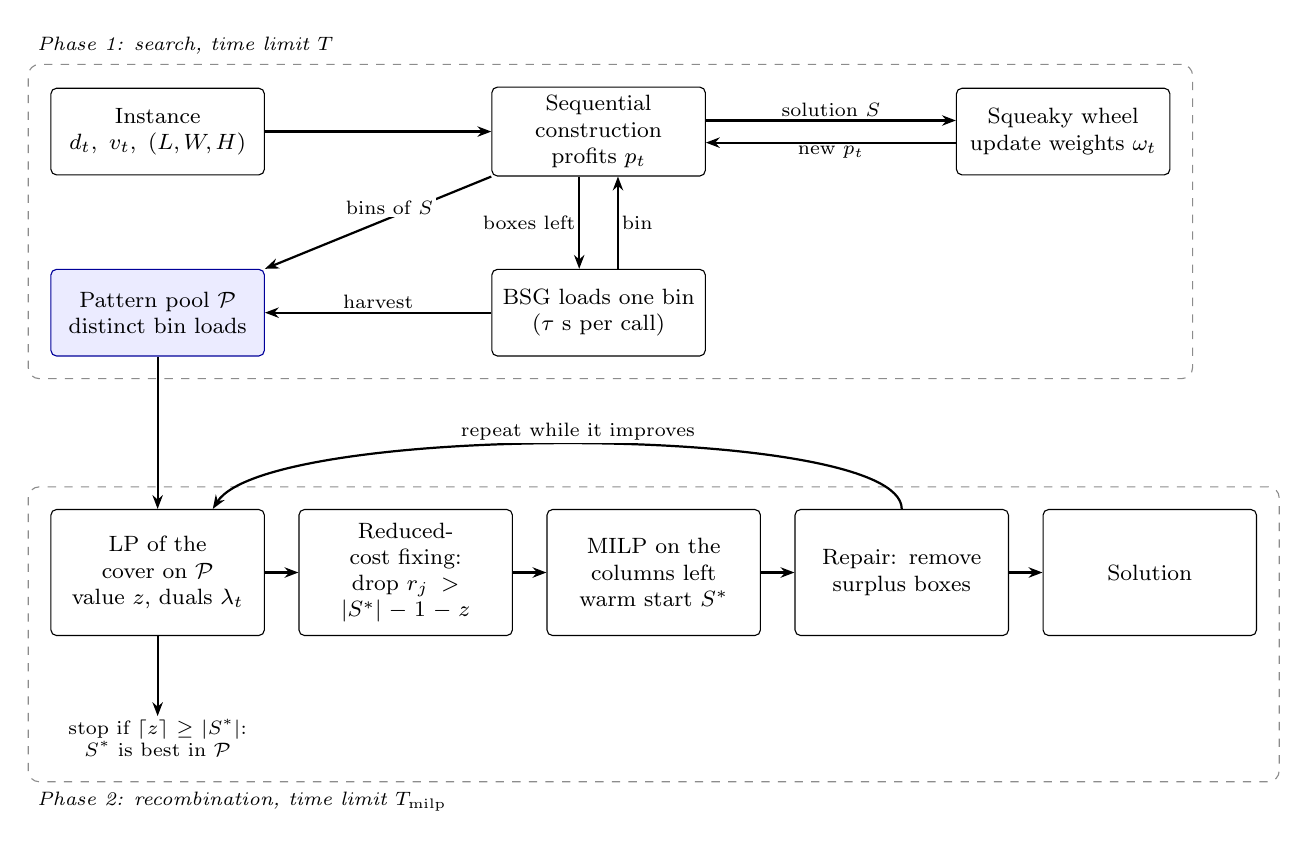
\begin{tikzpicture}[
  font=\footnotesize,
  box/.style={draw, rounded corners=2pt, align=center, minimum height=1.1cm, text width=2.5cm, fill=white, inner sep=3pt},
  pool/.style={box, fill=blue!8, draw=blue!60!black},
  box2/.style={box, minimum height=1.6cm},
  arr/.style={-{Stealth[length=5pt]}, thick},
  lab/.style={font=\scriptsize, fill=white, inner sep=1pt},
  phase/.style={draw=black!45, dashed, rounded corners=4pt, inner sep=8pt}
]
% Phase 1: search
\node[box]  (inst)   at (1.4,5.3)  {Instance\\ $d_t,\ v_t,\ (L,W,H)$};
\node[box]  (constr) at (7.0,5.3)  {Sequential construction\\ profits $p_t$};
\node[box]  (swo)    at (12.9,5.3) {Squeaky wheel\\ update weights $\omega_t$};
\node[box]  (bsg)    at (7.0,3.0)  {BSG loads one bin\\ ($\tau$ s per call)};
\node[pool] (pool)   at (1.4,3.0)  {Pattern pool $\mathcal{P}$\\ distinct bin loads};
\draw[arr] (inst) -- (constr);
\draw[arr] ([yshift=4pt]constr.east) -- node[lab,above]{solution $S$} ([yshift=4pt]swo.west);
\draw[arr] ([yshift=-4pt]swo.west) -- node[lab,below]{new $p_t$} ([yshift=-4pt]constr.east);
\draw[arr] ([xshift=-7pt]constr.south) -- node[lab,left]{boxes left} ([xshift=-7pt]bsg.north);
\draw[arr] ([xshift=7pt]bsg.north) -- node[lab,right]{bin} ([xshift=7pt]constr.south);
\draw[arr] (bsg.west) -- node[lab,above]{harvest} (pool.east);
\draw[arr] (constr.south west) -- node[lab,above,pos=0.45]{bins of $S$} (pool.north east);
% Phase 2: recombination
\node[box2] (lp)     at (1.4,-0.3)  {LP of the cover on $\mathcal{P}$\\ value $z$, duals $\lambda_t$};
\node[box2] (fix)    at (4.55,-0.3) {Reduced-cost fixing:\\ drop $r_j > |S^*|-1-z$};
\node[box2] (milp)   at (7.7,-0.3)  {MILP on the columns left\\ warm start $S^*$};
\node[box2] (rep)    at (10.85,-0.3){Repair: remove\\ surplus boxes};
\node[box2] (out)    at (14.0,-0.3) {Solution};
\draw[arr] (pool) -- (lp);
\draw[arr] (lp) -- (fix);
\draw[arr] (fix) -- (milp);
\draw[arr] (milp) -- (rep);
\draw[arr] (rep) -- (out);
\draw[arr] (rep.north) .. controls +(0,1.1) and +(0.7,1.1) .. ([xshift=0.7cm]lp.north)
  node[pos=0.5,lab,above]{repeat while it improves};
\node[lab,align=center,text width=2.5cm] (stop) at (1.4,-2.4) {stop if $\lceil z\rceil\ge|S^*|$:\\ $S^*$ is best in $\mathcal{P}$};
\draw[arr] (lp.south) -- (stop.north);
\begin{scope}[on background layer]
  \node[phase, fit=(inst)(constr)(swo)(bsg)(pool)] (ph1) {};
  \node[phase, fit=(lp)(fix)(milp)(rep)(out)(stop)] (ph2) {};
\end{scope}
\node[anchor=south west, font=\scriptsize\itshape] at (ph1.north west) {Phase 1: search, time limit $T$};
\node[anchor=north west, font=\scriptsize\itshape] at (ph2.south west) {Phase 2: recombination, time limit $T_{\mathrm{milp}}$};
\end{tikzpicture}
\caption{Overview of the method. The construction loads the bins one by one with BSG using the
profits $p_t$ of the box types; the squeaky wheel loop changes the profits from one construction
to the next. Every bin that BSG returns, and the best complete greedy loads that it explored
(harvest), are stored in the pool $\mathcal{P}$. The recombination phase solves the LP
relaxation of the set covering model over $\mathcal{P}$, removes the columns that cannot be in a
better solution and solves the remaining MILP, warm started with the best solution $S^*$.}
\label{fig:overview}
\end{figure}

\subsection{Notation}
\label{sec:m-notation}

The bins are identical, with dimensions $L\times W\times H$ and volume $V=LWH$. The $n$ boxes are
grouped into $m$ types of identical dimensions; type $t$ has volume $v_t$ and $d_t$ boxes, so
that $n=\sum_t d_t$. A \emph{load} is a set of boxes placed in a bin without overlaps, and its
\emph{pattern} is the vector $a\in\mathbb{Z}_{\ge 0}^{m}$ whose component $a_t$ is the number of
boxes of type $t$ in the load. A vector $a\le d$ is \emph{feasible} if there is a load with
pattern $a$. A solution $S$ is a list of loads whose patterns add up to $d$, and $|S|$ is the
number of bins. The search stops early when $|S|$ reaches the lower bound $\mathrm{LB}$ of
Section~\ref{sec:problem}.

\subsection{Loading one bin with BSG}
\label{sec:m-bsg}

Each bin is loaded by BSG, a beam search guided by a greedy algorithm \citep{Araya2014,Araya2017}
that places blocks of boxes in maximal free spaces. We summarise the elements that matter for
the rest of the method.

\paragraph{Blocks.}
A block is a cuboid arrangement of boxes that is placed as a unit. The blocks of one box are the
box in each allowed orientation, and further blocks are obtained by joining two blocks along the
$x$, $y$ or $z$ axis, as in \citet{Fanslau2010} and \citet{Araya2014}, so that every block has a
guillotine structure.
A joined block is kept if its boxes are still available, it fits in the bin, its boxes fill at
least a fraction $f_{\min}=0.98$ of its volume, and it differs from the blocks already generated.
The generation stops after $N_{\max}=500$ blocks.

\paragraph{Free spaces.}
The free volume of the bin is represented by the set of maximal free spaces \citep{Parreno2008}.
Every space is anchored at its corner closest to the origin of the bin, and the next space to be
filled is the one whose anchor is closest to the origin, with ties broken by larger volume. The
load therefore grows from one corner of the bin. An action places a block that fits in the
selected space at its anchor.

\paragraph{Evaluation of the blocks.}
The blocks that fit in the selected space are ranked with the VCS function of \citet{Araya2017},
in which the volume of the block is replaced by its profit:
\begin{equation}
\label{eq:vcs}
\mathrm{VCS}(b) = P(b)\,\bigl(1-\mathrm{loss}(b)\bigr)^{\beta}\,\mathrm{CS}_q(b)^{\alpha}\,|b|^{-\gamma}.
\end{equation}
Here $P(b)=\sum_t p_t\,\nu_t(b)$ is the profit of the block, where $\nu_t(b)$ is the number of boxes
of type $t$ in $b$ and $p_t$ is the profit of a box of type $t$ (Section~\ref{sec:m-construct});
$\mathrm{loss}(b)$ is the proportion of the free space that the remaining boxes cannot fill
after placing $b$, estimated with one-dimensional knapsack problems; $\mathrm{CS}_q(b)$ is the
proportion of the surface of $b$ in contact with placed blocks or walls, where a gap of at most
a proportion $q$ of the block dimension still counts as contact; and $|b|=\sum_t\nu_t(b)$ is the number of boxes
of $b$. We keep the values $\alpha=2.4407$, $\beta=2.2652$, $\gamma=0.3896$ and $q=0.0164$ that
were tuned for the container loading problem; we do not retune them for bin packing
(the sensitivity analysis is in Section~\ref{sec:e-ablation}).

\paragraph{Greedy and beam search.}
The greedy algorithm repeatedly selects the next free space and places in it the best ranked
block, until no block fits. The value of a complete load is the total profit of its boxes. BSG is
a beam search whose children are generated with the best ranked blocks for the selected space,
and each child is evaluated by the value of its greedy completion. The $B$ best children are kept
at each level, and the best complete load found by any greedy completion is returned. BSG is run
repeatedly with increasing effort until a time limit is reached \citep{Araya2017}: it starts with
$B=4$ and at most $C=16$ children per level, and after every run $B$ and $C/B$ are multiplied by
$\sqrt{2}$. The implementation applies the optimisations of \citet{Guesser2026}, which do not
change the result of the search.

In what follows, $\textsc{LoadBin}(R,p,\tau)$ denotes one such search of $\tau$ seconds over the multiset
of boxes $R$ with box profits $p$. It returns a load, its pattern $a\le R$, and the positions of
its boxes. The time $\tau$ covers the search and not the generation of the blocks, which costs a
fixed overhead of the order of two milliseconds per call. With very short limits BSG may end before completing
any greedy run; in that case one greedy run is completed without time limit, so that \textsc{LoadBin} always returns
a non-empty load when some box fits.

\subsection{Sequential construction with box profits}
\label{sec:m-construct}

The construction (Algorithm~\ref{alg:construct}) fills the bins one at a time. In each step
BSG loads a bin with the boxes that are still unplaced, and the boxes that it places are removed
from the instance. The loader is guided by profits instead of volumes. The profit of a box of
type $t$ is
\begin{equation}
\label{eq:profit}
p_t \;=\; V\left(\frac{v_t}{V}\right)^{\kappa},\qquad \kappa\ge 1 .
\end{equation}
With $\kappa=1$ the profit is the volume, and BSG maximises the filling of each bin. With
$\kappa>1$ a large box is worth more than its volume, so a bin that holds one more large box is
preferred to a bin with the same volume made of small boxes. Large boxes are thus loaded first
and the small ones, which fill the gaps best, remain for the bins that follow. We use $\kappa=2$ in all the experiments.

\begin{algorithm}[t]
\caption{$\textsc{Construct}(p)$}
\label{alg:construct}
\begin{algorithmic}[1]
\Require box profits $p$, demands $d$, time per bin $\tau$
\Ensure a solution $S$
\State $R\gets d$;\quad $S\gets\emptyset$
\While{$R\neq 0$}
  \State $(\ell,a)\gets \textsc{LoadBin}(R,p,\tau)$ \Comment{BSG, profit-guided}
  \State store $a$ in the pool $\mathcal{P}$ \Comment{with the positions of $\ell$}
  \State $R\gets R-a$;\quad append $\ell$ to $S$
\EndWhile
\State \Return $S$
\end{algorithmic}
\end{algorithm}

\subsection{Squeaky wheel optimisation of the box profits}
\label{sec:m-swo}

A single construction leaves a few bins with little load, usually the last ones, and which box
types end up there depends on the profits. Squeaky wheel optimisation \citep{Joslin1999} repeats
a construction, analyses the result, and raises the priority of the elements that were
troublesome. Here the elements are the box types, and the troublesome ones are those found in
the least loaded bins: they were hard to combine into well filled bins. Algorithm~\ref{alg:swo}
describes the loop.

Let $\omega_t$ be a weight of type $t$, initially one, so that the profit used in a construction is
$\omega_t\,p_t$ with $p_t$ from \eqref{eq:profit}. After each construction, the types that appear in
the $\max\{1,\mathrm{round}(0.1\,|S|)\}$ least loaded bins of that solution have their weight multiplied by
$1+\rho$, with $\rho=0.3$. Then every weight is multiplied by $e^{\varepsilon_t}$, where
$\varepsilon_t$ is drawn from a normal distribution with mean zero and standard deviation
$\sigma=0.05$. The weights accumulate along the iterations; they are neither reset nor decayed.
The noise breaks ties between types that are always treated alike and makes consecutive
constructions differ even when the set of troublesome types does not change.

The incumbent $S^*$ is replaced by a new solution when the latter has fewer bins or the same
number of bins and a smaller volume in its least loaded bin; the second criterion prefers
solutions that are closer to losing a bin. The loop ends when $|S^*|=\mathrm{LB}$ or when the
time limit $T$ is reached. The iteration in progress is completed, so the limit can be exceeded
by the duration of one construction.

\begin{algorithm}[t]
\caption{Squeaky wheel optimisation}
\label{alg:swo}
\begin{algorithmic}[1]
\Require instance, $\kappa$, $\rho$, $\sigma$, time limit $T$
\Ensure incumbent $S^*$ and pool $\mathcal{P}$
\State $\omega_t\gets 1$ for all $t$;\quad $S\gets \textsc{Construct}(p)$;\quad $S^*\gets S$
\While{$|S^*|>\mathrm{LB}$ \textbf{and} time $<T$}
  \State $M\gets$ the $\max\{1,\mathrm{round}(0.1\,|S|)\}$ least loaded bins of $S$
  \ForAll{types $t$}
    \If{some bin of $M$ contains a box of type $t$} $\omega_t\gets(1+\rho)\,\omega_t$ \EndIf
    \State $\omega_t\gets \omega_t\,e^{\varepsilon_t}$,\quad $\varepsilon_t\sim\mathcal{N}(0,\sigma^2)$
  \EndFor
  \State $S\gets \textsc{Construct}(\omega\cdot p)$
  \If{$S$ is better than $S^*$} $S^*\gets S$ \EndIf
\EndWhile
\State \Return $S^*$, $\mathcal{P}$
\end{algorithmic}
\end{algorithm}

\subsection{Pattern pool and harvest}
\label{sec:m-pool}

Every bin returned by \textsc{LoadBin} during the construction and the squeaky wheel loop is
stored in the pool $\mathcal{P}$. A pattern is stored once, whichever iteration produced it, and
the pool keeps the positions of the boxes of the first load found with that pattern. A pattern
in the pool is therefore always feasible, and a load is available for it.

\paragraph{Harvest.}
Each call to BSG executes many greedy completions, and each of them is a complete load of a bin,
but only the best one is returned. The harvest keeps some of the others. BSG notifies a callback
after every greedy completion. The callback computes the occupied volume $\upsilon$ of the
completed load and updates $\upsilon^*$, the largest volume seen in the current call. A load is
retained as a candidate if $\upsilon\ge\theta\,\upsilon^*$ and its pattern is neither in the pool
nor among the candidates. When the call ends, the candidates that still satisfy
$\upsilon\ge\theta\,\upsilon^*$ for the final value of $\upsilon^*$ are sorted by volume, and the
$K$ most loaded are added to the pool. To bound memory, when the candidates exceed $8K$ during the
call only the $K$ most loaded are kept. We use $K=10$ and $\theta=0.95$. The harvested loads are produced under the same state as
the load that BSG returns, with the same unplaced boxes, so they are valid columns for the covering
model, although the construction does not use them. The harvest acts whenever BSG loads an empty bin; it is not applied when BSG reloads a bin with
fixed boxes in the improvement phase of Appendix~\ref{app:improve}. The loads of the final solution are also added to the pool before the recombination.

The harvest does not alter any decision of BSG; it only records loads that BSG has already built,
at the cost of some extra time per call. Its effect is on the pool, which fills much faster per
second of search. This matters for short time limits, where the squeaky wheel loop alone would
produce too few patterns for the recombination to find a better combination
(Section~\ref{sec:e-ablation} isolates the effect of the harvest).

\subsection{Recombination by set covering or partitioning}
\label{sec:m-cover}

Let the columns $j\in\mathcal{P}$ be the patterns of the pool, with $a_{tj}$ boxes of type $t$ in
pattern $j$. The recombination solves
\begin{align}
\min\ & \sum_{j\in\mathcal{P}} x_j \label{eq:obj}\\
\text{s.t.}\ & \sum_{j\in\mathcal{P}} a_{tj}\,x_j \ge d_t \quad \forall t, \label{eq:cover}\\
& x_j\in\mathbb{Z}_{\ge 0}\quad\forall j, \label{eq:int}
\end{align}
where $x_j$ is the number of bins loaded with pattern $j$. The constraints are covering rather than
partitioning constraints: a combination of patterns may contain a box type more often than
demanded, and the surplus boxes are removed afterwards (see the repair step below). Variables are
general integers because the same pattern can be used in several bins. When removing a box can make
a load infeasible, as with vertical support (Section~\ref{sec:m-ext}), \eqref{eq:cover} is
replaced by the equalities $\sum_j a_{tj}x_j=d_t$ (\emph{partitioning model}); no box is then
removed and the repair step is not needed.

\paragraph{LP relaxation and pool bound.}
Let $z$ be the optimal value of the LP relaxation of \eqref{eq:obj}--\eqref{eq:int} and
$\lambda$ an optimal dual solution, with one price $\lambda_t$ per box type ($\lambda\ge 0$ in the
covering model, free in the partitioning model). The reduced
cost of column $j$ is
\begin{equation}
\label{eq:rc}
r_j \;=\; 1-\sum_t a_{tj}\,\lambda_t \;\ge\; 0 .
\end{equation}

\begin{proposition}
\label{prop:fix}
(i) Every solution of \eqref{eq:obj}--\eqref{eq:int} has at least $\lceil z\rceil$ bins.
(ii) If a solution has at most $U$ bins, then $x_j=0$ for every column $j$ with $r_j>U-z$.
\end{proposition}
\begin{proof}
Let $x$ be feasible. Using \eqref{eq:rc}, then $\lambda\ge 0$ together with \eqref{eq:cover}, and
finally strong duality ($z=\sum_t\lambda_t d_t$),
\[
\sum_j x_j=\sum_j r_j x_j+\sum_t\lambda_t\sum_j a_{tj}x_j\;\ge\;\sum_j r_j x_j+\sum_t\lambda_t d_t
\;=\;z+\sum_j r_j x_j .
\]
In the partitioning model the inequality is an equality and $\lambda\ge 0$ is not needed. Since
$r_j\ge 0$, $\sum_j x_j\ge z$, and the left side is an integer, which gives (i). If
$\sum_j x_j\le U$, the inequality gives $r_jx_j\le U-z$ for every $j$, so $x_j\ge 1$ requires
$r_j\le U-z$, which gives (ii).
\end{proof}

Part (ii) is reduced-cost fixing \citep{Wolsey1998}. The proposition is stated for the
columns of the pool. It says nothing about patterns that the pool does not contain, so $\lceil
z\rceil$ is a bound on what the pool can offer and not a lower bound on the optimum of the
instance.

\paragraph{Procedure.}
Algorithm~\ref{alg:recombine} starts from the incumbent $S^*$ of the search and looks for a
solution with at most $U=|S^*|-1$ bins. The patterns of $S^*$ are added to the pool, and the LP is
solved. If $\lceil z\rceil\ge|S^*|$, part (i) shows that the pool holds no better solution and
the procedure stops, which makes the MILP unnecessary
(Section~\ref{sec:e-recomb} reports in which fraction of the runs this happens). Otherwise, the
columns with $r_j>U-z$ are removed by part (ii) and the MILP is solved on the remaining columns
plus the columns of $S^*$, which are kept so that $S^*$ gives a feasible starting point for the
solver. The MILP returns an integer vector $x$, from which the repair step builds a solution. If
that solution has fewer bins than $S^*$, it becomes the new incumbent and the procedure starts
again with the new $U$; otherwise the procedure stops. The time limit $T_{\mathrm{milp}}$ is shared
by all the repetitions.

\paragraph{Repair.}
Given $x$, take $x_j$ copies of the load of every pattern $j$ with $x_j>0$. For each type $t$ with
a surplus $e_t=\sum_j a_{tj}x_j-d_t>0$, remove $e_t$ boxes of that type, taking them from the
copies that come last in a fixed order. The loads that become empty are discarded. A load that
loses a box remains feasible, because removing a box cannot create an overlap, so the result is a
valid solution with at most $\sum_j x_j$ bins. This holds only when no box needs another box below it;
with a vertical support requirement the removal could leave a box without support, and the
partitioning model is used instead (Section~\ref{sec:m-ext}).

\begin{algorithm}[t]
\caption{$\textsc{Recombine}(S^*,\mathcal{P},T_{\mathrm{milp}})$}
\label{alg:recombine}
\begin{algorithmic}[1]
\Require incumbent $S^*$, pool $\mathcal{P}$, time limit $T_{\mathrm{milp}}$
\Ensure a solution with $|S|\le|S^*|$
\State add the patterns of $S^*$ to $\mathcal{P}$;\quad $S\gets S^*$
\Loop
  \State solve the LP relaxation of \eqref{eq:obj}--\eqref{eq:int} on $\mathcal{P}$; get $z$ and $\lambda$
  \If{$\lceil z\rceil\ge|S|$} \State \Return $S$ \Comment{pool bound (i)}
  \EndIf
  \State $U\gets|S|-1$
  \State $\mathcal{P}'\gets\{j: r_j\le U-z\}\ \cup$ columns of $S$ \Comment{fixing (ii)}
  \State solve \eqref{eq:obj}--\eqref{eq:int} on $\mathcal{P}'$ with warm start $S$ within the time left; get $x$
  \State $S'\gets\textsc{Repair}(x)$
  \If{$|S'|<|S|$} $S\gets S'$ \Else \State \Return $S$ \EndIf
\EndLoop
\end{algorithmic}
\end{algorithm}

\begin{figure}[t]
\centering
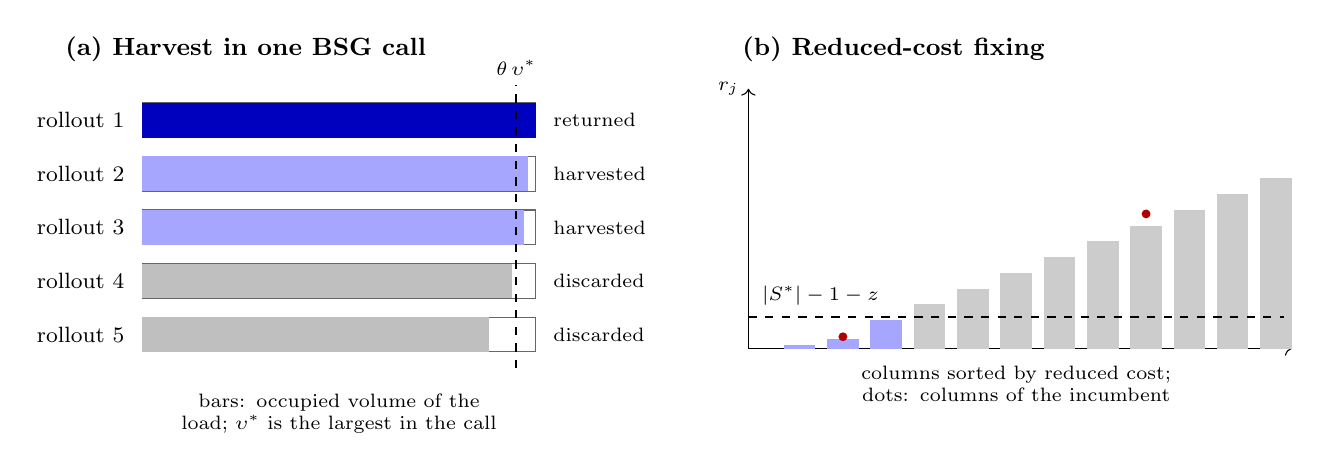
\begin{tikzpicture}[font=\footnotesize]
% (a) harvest in one BSG call
\node[font=\small\bfseries, anchor=west] at (0,4.2) {(a) Harvest in one BSG call};
\foreach \k/\vv/\col/\lbl in {0/100/blue!75!black/{returned},1/98/blue!35/{harvested},2/97/blue!35/{harvested},3/94/black!25/{discarded},4/88/black!25/{discarded}}{
  \pgfmathsetmacro{\yy}{3.3-0.68*\k}
  \node[anchor=east] at (1.0,\yy) {rollout \the\numexpr\k+1\relax};
  \draw[black!60] (1.1,\yy-0.22) rectangle (6.1,\yy+0.22);
  \pgfmathsetmacro{\bw}{1.1+5*\vv/100}
  \fill[\col] (1.1,\yy-0.22) rectangle (\bw,\yy+0.22);
  \node[anchor=west, font=\scriptsize] at (6.2,\yy) {\lbl};
}
\draw[dashed, thick] (5.85,0.15) -- (5.85,3.75);
\node[font=\scriptsize, anchor=south] at (5.85,3.75) {$\theta\,\upsilon^*$};
\node[font=\scriptsize, anchor=north, text width=6.2cm, align=center] at (3.6,-0.05) {bars: occupied volume of the load; $\upsilon^*$ is the largest in the call};
% (b) reduced-cost fixing
\node[font=\small\bfseries, anchor=west] at (8.6,4.2) {(b) Reduced-cost fixing};
\draw[->] (8.8,0.4) -- (8.8,3.7) node[left, font=\scriptsize] {$r_j$};
\draw[->] (8.8,0.4) -- (15.7,0.4);
\foreach \q/\rv in {1/0.1,2/0.3,3/0.9,4/1.4,5/1.9,6/2.4,7/2.9,8/3.4,9/3.9,10/4.4,11/4.9,12/5.4}{
  \pgfmathsetmacro{\xx}{8.9+0.55*\q}
  \pgfmathsetmacro{\hh}{0.4*\rv}
  \ifnum\q<4
    \fill[blue!35] (\xx-0.2,0.4) rectangle (\xx+0.2,0.4+\hh);
  \else
    \fill[black!20] (\xx-0.2,0.4) rectangle (\xx+0.2,0.4+\hh);
  \fi
}
\draw[dashed, thick] (8.8,0.8) -- (15.6,0.8);
\node[font=\scriptsize, anchor=south west] at (8.85,0.82) {$|S^*|-1-z$};
\fill[red!70!black] (8.9+0.55*2,0.55) circle (1.6pt);
\fill[red!70!black] (8.9+0.55*9,0.4+0.4*3.9+0.15) circle (1.6pt);
\node[font=\scriptsize, anchor=north, text width=7cm, align=center] at (12.2,0.3) {columns sorted by reduced cost; dots: columns of the incumbent};
\end{tikzpicture}
\caption{Schematic of two elements of the method (the values are illustrative). (a) One call to
BSG executes several greedy completions. The best one is returned to the construction, and the
others whose volume reaches $\theta\,\upsilon^*$ are added to the pool, up to $K$ of them. (b)
After the LP of the cover is solved, the columns whose reduced cost exceeds $|S^*|-1-z$ cannot be
in a solution with fewer bins than the incumbent and are removed (grey). The columns of the
incumbent stay in the model as the warm start, even when their reduced cost is above the threshold.}
\label{fig:harvest-fixing}
\end{figure}

\subsection{Overall algorithm}
\label{sec:m-overall}

Algorithm~\ref{alg:overall} puts the two phases together. Phase 1 spends the time limit $T$ on the
squeaky wheel loop, which builds the incumbent and fills the pool; Phase 2 spends at most
$T_{\mathrm{milp}}$ on the recombination. The time limits are independent, so the total running time
is about $T+T_{\mathrm{milp}}$, less when the lower bound is reached in Phase 1 or the pool bound
stops Phase 2. The result is checked box by box before it is reported.
The reduced costs used for the fixing are those that the LP solver returns at the optimum.

\begin{algorithm}[t]
\caption{Overall method}
\label{alg:overall}
\begin{algorithmic}[1]
\Require instance, $\kappa$, $\tau$, $K$, $T$, $T_{\mathrm{milp}}$
\Ensure a solution $S$
\State $(S^*,\mathcal{P})\gets$ squeaky wheel optimisation with time limit $T$ \Comment{Algorithm~\ref{alg:swo}, harvest with $K$}
\If{$T_{\mathrm{milp}}>0$ \textbf{and} $|S^*|>\mathrm{LB}$}
  \State $S\gets\textsc{Recombine}(S^*,\mathcal{P},T_{\mathrm{milp}})$ \Comment{Algorithm~\ref{alg:recombine}}
\Else
  \State $S\gets S^*$
\EndIf
\State check that $S$ is a valid packing of all the boxes
\State \Return $S$
\end{algorithmic}
\end{algorithm}

\subsection{Properties}
\label{sec:m-prop}

\paragraph{Validity and monotonicity.}
Every load that the method returns is a load that BSG built, possibly with some boxes removed
by the repair step, and the final check verifies box by box that the loads lie inside the bin, do
not intersect, and contain every box exactly once. The recombination starts from $S^*$, so it
never returns more bins than the search found.

\paragraph{What is guaranteed.}
When the LP bound stops the procedure, the incumbent is optimal \emph{for the pool}. The method
does not prove that it is optimal for the instance, and it does not search for patterns that are
not in the pool. Its quality depends on how well the construction and the harvest cover the
patterns that a good solution needs.

\paragraph{Cost.}
A construction needs one BSG call per bin, so it takes about $|S|\,(\tau+\delta)$ seconds, where
$\delta$ is the fixed overhead per call, and the squeaky wheel loop repeats it until the time
limit. The recombination adds the time of one LP and, when the LP bound does not stop it, of the
MILP, both bounded by $T_{\mathrm{milp}}$; HiGHS \citep{Huangfu2018} runs on a single thread.
The harvest adds the cost of one comparison of patterns per greedy completion.

\paragraph{Early stop by the pool bound.}
The implementation has an option that solves the LP of the pool every two seconds during the
squeaky wheel loop, once the first six seconds have passed. When $\lceil z\rceil\ge|S^*|$ it stops
the loop after $z$ has not decreased by more than $0.01$ in six seconds, so that $T$ becomes a
maximum, and when $\lceil z\rceil<|S^*|$ it tries the recombination at that point. We do not use the option in
the experiments of this paper, because the comparisons keep the time limits fixed.

\subsection{Rotations and vertical support}
\label{sec:m-ext}

\paragraph{Rotations.}
With rotations allowed, the generation of blocks includes the six orientations of every box. This
is the only change: the construction, the squeaky wheel loop, the pool and the recombination do
not depend on the orientation, because a pattern only counts boxes per type. The lower bound
used to stop the search is the continuous bound.

\paragraph{Vertical support.}
With the support requirement of Section~\ref{sec:problem}, only BSG and the recombination change.
Inside a block, one sub-block is stacked on another only if the lower one has a flat top that
covers the whole base of the upper one. A block placed above the floor is accepted only if every
box of its bottom layer has at least a fraction $0.7$ of its base area resting directly on the top
faces of the boxes below. The check is made when a block is placed, so every load that BSG returns,
and every harvested load, satisfies it. The recombination uses the partitioning model, so that no
box is removed from a load. The rest of the method is unchanged.
We tested the whole pipeline (squeaky wheel loop, harvest and partitioning recombination) on the industrial instances. The recombination did not improve any run there, and the construction alone with $\tau=2$ s and $\kappa=1$
is the better configuration for the large instances, and the loop alone for the small ones (Section~\ref{sec:e-ind}).

\subsection{Parameters and configurations}
\label{sec:m-params}

Table~\ref{tab:params} lists the parameters of the method, and Table~\ref{tab:configs} the three
configurations used in the experiments. They differ in the time limits of the search and of the
recombination, in the time per bin, and in whether the harvest is active. For a short search the
harvest compensates for the small number of squeaky wheel iterations; for a long search the
pool already holds many patterns without it.
With three seeds, \cfgqual{} with the harvest gives $7250.0\pm 1.0$ against $7249.3\pm 1.2$ without it ($p=0.72$), which supports leaving it out (Section~\ref{sec:e-mpv}).
The values of $\kappa$, $\rho$, $\sigma$, $\theta$ and $K$ were chosen on the original instances, and the sensitivity to $\rho$, $\sigma$, the fraction of least loaded bins, $K$, $\theta$ and $\tau$ is reported in Section~\ref{sec:e-ablation}.
\pend{Decide whether the noise $\sigma$ and the harvest threshold $\theta$ stay in the method. In the sensitivity analysis
(72 original instances, \cfgfast{}) $\sigma=0$ and $\theta=0.8$ were not worse than the defaults ($-2.0$ bins each, not
significant), so both could be removed (no noise; harvest the $K$ most loaded distinct loads without threshold). Confirm
with $\sigma=0$ and with $\theta=0$ on the 240 original instances and on the blind set before removing them.}
The method is implemented in C++ on top of the
Metasolver framework, with HiGHS 1.15.1 as the LP and MILP solver; the recombination is
compiled only when HiGHS is available. The implementation is available at \url{https://github.com/NicoFuentese/Metasolver} (branch \texttt{nico/bpp-mejoras}).

\begin{table}[t]
\centering
\caption{Parameters introduced by the method and the values used in all the experiments; the harvest size $K$ and the
time limits are part of the configurations (Table~\ref{tab:configs}). The parameters of BSG keep the values tuned for the
container loading problem \citep{Araya2017} and are given in Section~\ref{sec:m-bsg}; the minimum support of 70\% is part
of the problem (Section~\ref{sec:problem}).}
\label{tab:params}
\begin{tabular}{@{}llr@{}}
\toprule
Parameter & Symbol & Value\\
\midrule
Profit exponent & $\kappa$ & $2$\\
Weight increase of the types in the least loaded bins & $\rho$ & $0.3$\\
Standard deviation of the log-normal noise & $\sigma$ & $0.05$\\
Fraction of least loaded bins analysed & & $0.1$\\
Harvest threshold & $\theta$ & $0.95$\\
\bottomrule
\end{tabular}
\end{table}

\begin{table}[t]
\centering
\caption{Configurations. $T$: time limit of the squeaky wheel loop; $\tau$: BSG time per bin;
$K$: bins harvested per BSG call; $T_{\mathrm{milp}}$: time limit of the recombination, which adds to $T$.}
\label{tab:configs}
\begin{tabular}{@{}lrrrr@{}}
\toprule
Configuration & $T$ (s) & $\tau$ (s) & $K$ & $T_{\mathrm{milp}}$ (s)\\
\midrule
\cfgfast{}   & 4   & 0.005 & 10 & 30\\
\cfgbal{}  & 20  & 0.005 & 10 & 60\\
\cfgqual{} & 100 & 0.02  & 0  & 100\\
\bottomrule
\end{tabular}
\end{table}

% Seccion de experimentos del paper de bin packing 3D (BSG_BPP), organizada por preguntas.
% Las cifras vienen de AGENTS.md (secciones 14-24) y del README; \pend marca lo pendiente.
\providecommand{\pend}[1]{\textcolor{red}{[PENDING: #1]}}

\section{Computational experiments}
\label{sec:experiments-bpp}

The experiments answer the following questions. How does the method compare with the literature on the
benchmark of \citet{Martello2000} with fixed orientation (Section~\ref{sec:e-mpv}) and with rotations
(Section~\ref{sec:e-rot})? What does each component contribute (Section~\ref{sec:e-ablation})? How does the
recombination behave, and when is the LP of the pool enough (Section~\ref{sec:e-recomb})? Do the effects hold on
instances that were not used to design the method (Section~\ref{sec:e-heldout})? Does the same pipeline work with
vertical support (Section~\ref{sec:e-ind})? Where are its limits (Section~\ref{sec:e-scale})?
Section~\ref{sec:e-setup} describes the instances, the machine and the protocol, and
Section~\ref{sec:e-discussion} states what the evidence supports and where it is weak. The variants that we tried
and discarded are listed in Appendix~\ref{app:negative}. All the solutions reported were checked by an independent validator.
\pend{Generate every table and figure of this section with a script from the raw result files, instead of
transcribing the numbers from the project notes.}

\subsection{Experimental setup}
\label{sec:e-setup}

\paragraph{Instances.}
The benchmark of \citet{Martello2000} has eight classes of instances. For each class there are
instances with $n\in\{50,100,150,200\}$ boxes, ten per size, so that a class has 40 instances and
the benchmark 320. The bins are cubes of side 100 in classes 1--5 and 8, of side 10 in class 6 and
of side 40 in class 7. Several authors report a separate total for classes 1 and 4--8 (240 instances) besides the total for all the classes, and we do the same. We used these 240 instances, and sets of generated instances, to
design the method and to choose the configurations; they are therefore not independent of the
design. Classes 2 and 3 (80 instances) were never used to choose anything and serve as held-out
set. In addition we generated instances with the distribution of the benchmark, from its
description and not with the original generator. A first set of 240 instances (classes 1 and
4--8, ten per size) was used for exploration, in particular for the exponent $\kappa$ and the
parameters of BSG. A second set has 320 instances with a new seed (eight classes, four sizes,
ten instances per cell); instances 1 to 6 of every cell were used to test options that are not part of the method, and instances 7 to 10 of every cell (128 instances) were not used in any
decision and form a blind set. The files of this blind set were not preserved, so for the measurements of Section~\ref{sec:e-recomb} we generated a second blind set of 128 instances (eight classes, four sizes,
four instances each) with the same generator and new seeds, $9\,000\,000+10^6c+1000n+i$ for class $c$, $n$ boxes and instance $i$; no decision depends on it.

The industrial instances are the 160 files of the collection that accompanies the benchmark of
\citet{Elhedhli2019}: four classes, eight sizes ($n\in\{50,100,150,200,500,1000,1500,2000\}$) and
five instances per cell, with the dimensions of the boxes in millimetres. The files do not include
the dimensions of the pallet; we use $1200\times 800\times 2055$ mm, the dimensions that
\citet{Elhedhli2019} state for their data sets. The files have the same distribution, quantity and
structure as the instances of that article, and the lower bound by volume of each cell agrees with
the lower bound they report in 30 of the 32 cells; but we could not verify that the instances are the
same, and their numbering differs. For the comparison we therefore use the mean over the five instances of each cell.
We also built 72 additional industrial instances: 48 by resampling the boxes of the four classes
(three instances for each class and for $n=500,1000,1500,2000$) and 24 with $n\in\{500,1000,1500\}$ from the product
catalogue that comes with the collection (eight instances per size). The first 48 come from the same
distribution as the original ones; the catalogue ones do not.

\paragraph{Implementation and machine.}
The method is implemented in C++ (g++ 16.2, \texttt{-O3}, C++11) on the Metasolver framework,
with HiGHS 1.15.1 \citep{Huangfu2018} on a single thread. All the experiments ran on the same machine,
an Intel Core i5-14400 (10 cores, 16 threads) under Windows 11. Each run is a separate process of the single-threaded
program. The time reported is the wall-clock time measured with the C function
\texttt{clock}, which on Windows is not CPU time; it includes the search, the recombination
and the generation of blocks. The time limit $T$ is checked between constructions
(Section~\ref{sec:m-swo}), so a run can exceed it by the duration of one construction.
On Linux, \texttt{clock} measures CPU time; the current version of the code measures $T$ and $T_{\mathrm{milp}}$ with a
monotonic wall clock (\texttt{std::chrono::steady\_clock}) and also gives a time limit to the LP of the pool, which the
version used in the campaigns of this paper did not have.

\paragraph{Conditions of the campaigns.}
Because the time limits are wall-clock limits, the amount of search that a run receives depends on the load of the machine, and the totals of two campaigns run under different loads
are not directly comparable. The repetition campaigns therefore follow one protocol: four runs in parallel at below-normal priority, one campaign at a time, so that two campaigns never share the machine.
Inside a campaign all the configurations that are compared use the same binary, the same instances and the same seeds, and the configurations of one instance are run one after the other by the same worker.
The comparisons between configurations are made inside a campaign and are paired by instance. Table~\ref{tab:e-conditions} lists the campaigns that follow this protocol and keep their raw files.
The earlier campaigns, marked with $^\dagger$, ran on the same machine with between two and five runs in parallel (the number was not recorded for a few of them), some at normal priority, and with earlier builds of the code,
some of which solved the MILP stage without the LP proof and the fixing of Section~\ref{sec:m-cover}; their raw files were not kept. We are repeating them under the protocol above, and until then the figures that come from them are
indicative and are not compared in absolute terms with those of the repetition.

\begin{table}[t]
\centering
\small\setlength{\tabcolsep}{3pt}
\caption{Campaigns that follow the protocol of the paper and keep their raw files (same machine, below-normal priority, one campaign at a time). Seeds: values of the seed of the program (1, 2, 3).}
\label{tab:e-conditions}
\begin{tabular}{@{}p{3.1cm}p{2.2cm}p{3.9cm}p{0.9cm}p{1.6cm}p{1.8cm}@{}}
\toprule
Used in & Instances & Configurations & Seeds & Parallel runs & Raw files\\
\midrule
Tables~\ref{tab:e-main}, \ref{tab:e-within}, \ref{tab:e-time} and \ref{tab:e-harvest} & 240 original (classes 1, 4--8) & \cfgfast{}, \cfgfast{} without harvest, \cfgbal{} & 1--3 & 4 & kept\\
\addlinespace
Tables~\ref{tab:e-main} and \ref{tab:e-budget} (\cfgqual{}) & 240 original & \cfgqual{} & 1--3 & 4 & kept\\
\addlinespace
Table~\ref{tab:e-recomb} & 128 generated (second blind set) & \cfgfast{}, \cfgfast{} without harvest, \cfgbal{}, \cfgbal{} with plain MILP, squeaky wheel alone & 1 & \pendshort{?} & kept\\
\bottomrule
\end{tabular}
\end{table}

\paragraph{Evaluation protocol.}
Each configuration is run with several seeds. The seed changes the noise of the squeaky wheel loop and the random choices of the improvement phase; the construction itself is deterministic except for the
effect of the clock on BSG. We report the total number of bins over the instances of a set, as the literature does, and the mean and the sample standard deviation of that total over the seeds. Three seeds
(1--3) are used for the configurations on the 240 original instances, on the first blind set and, for the shorter configurations, on classes 2 and 3 (the configuration of 33 s uses five seeds there); the ablation uses two seeds, and the second blind set and several budgets use a single seed, which
we indicate in each table. Two configurations are compared by the number of instances in which each is better and by the two-sided Wilcoxon signed-rank test on the differences in bins per instance. When
a single $p$-value is given for several seeds, it is computed on the mean of each instance over the seeds; otherwise the seed is indicated.
\pend{Declare which tests are confirmatory (samples independent of the design) and which are exploratory, or
correct for multiple comparisons (Holm). Add the raw files of the campaigns of November 2026 (\cfgfast{},
\cfgbal{}, \cfgqual{}) to the repository: they are cited as stored but are not in \texttt{results/bpp}, and record
the commit and the checksum of the executable of every campaign.}

The $p$-values and standard deviations of the repetition of \cfgfast{}, \cfgfast{} without harvest and \cfgbal{} on the 240 original instances (three seeds, four runs in parallel, no invalid solution and no error) were computed from its stored files.
For the earlier campaigns, those whose files were kept (classes 2 and 3, the first set of generated instances, the prototype run on the original instances in Table~\ref{tab:e-milp} and the experiment on large instances) were recomputed in the same way, and the
others come from the first analysis of each campaign because the raw files were lost (the first blind set, the rotations with three seeds and the ablation). \cfgqual{} on the original instances was also repeated (three seeds, four runs in parallel, no invalid solution and no error) and its figures come from its stored files. The controls without recombination
(``squeaky wheel alone'') use the same code with a time limit $T$ equal to the mean time of the configuration they are compared with.
\pend{repeat the rotation campaigns and the ablation saving the raw files, or keep this caveat}

\paragraph{Reproducibility.}
Every run has the form
\begin{center}\small\texttt{BSG\_BPP <instance file> -i <k> --seed <s> -o <solution file>}\end{center}
followed by the options of Table~\ref{tab:e-commands} (Appendix~\ref{app:tables}), where $k$ selects the instance inside the file and the seed
controls the noise of the squeaky wheel loop and the random choices of the improvement phase (the default is 1). \cfgqual{} keeps the default $\tau=0.02$ s, and \texttt{--rot} is added when the six orientations are allowed. The controls without recombination use the same command with \texttt{--milp} removed and $T$ set to the
time indicated. The files of the industrial instances are converted to the input format of the program, whose first line gives the number
of boxes and the dimensions of the pallet (1200, 800 and 2055).
The program is compiled with g++ 16.2 at \texttt{-O3} in the UCRT64 environment of MSYS2 and linked with HiGHS 1.15.1. Every solution is checked by a Python script that shares no code with the solver
(\texttt{validate\_bpp.py} in the repository, which verifies that the boxes lie inside the bin, do not intersect and that every box appears exactly once, with rotations when applicable) and,
for the industrial instances, by a second script that also verifies the support of every box
(the same script with the option \texttt{--support 0.7}).
\pend{Add the conversion of the industrial instances and the scripts of the campaigns other than the ablation
(\texttt{run\_ablation.sh}) to the repository or to a supplementary file.}

\paragraph{Results from the literature.}
We compare with the totals published for classes 1 and 4--8 without rotation: the column generation
of \citet{Mahvash2018} (Intel at 2.2~GHz, with CPLEX; their tables without rotation report no time, and
with rotation the time per instance goes from a few seconds to under 1000 s), the BRKGA of
\citet{Goncalves2013} (Intel i7-2630QM at 2~GHz, parallel evaluation, up to 130.6 s per instance), the space defragmentation of
\citet{Zhu2012SD} (30 s per instance) and the column generation over layers of \citet{Elhedhli2019}
(Intel i7-5500U at 2.4~GHz, 3.17 s per instance on average), together with the other methods in Table~8 of
\citet{Goncalves2013}. The numbers are the sums over cells of the published averages times ten. The machines
and the number of runs differ from ours, so the times are not comparable one to one.
To compare times we scale them by the single-thread rating of PassMark \citep{PassMark}: 3740 for our i5-14400,
1215 for the i7-2630QM of BRKGA and 1649 for the i7-5500U of LCGA. The limit of 130.6 s of BRKGA corresponds to
about 42 s on our machine (factor 3.1), although BRKGA evaluates its population in parallel, so the factor
underestimates its computing power. \citet{Mahvash2018} do not report times without rotation, and the machine of
\citet{Zhu2012SD} is not recorded.
\pend{Confirm the rating of the i5-14400 (PassMark shows 3700 for the i5-14400F; the 3740 of the draft is not
verified), mark the scaled times in Figure~\ref{fig:e-curve}, and ask the authors of \citet{Goncalves2013} and
\citet{Mahvash2018} for results per instance, which would allow paired tests.}
\subsection{Comparison with the literature, fixed orientation}
\label{sec:e-mpv}

Table~\ref{tab:e-main} compares three configurations of the method (Table~\ref{tab:configs}) with the
literature on classes 1 and 4--8. The fast configuration \cfgfast{}, which runs 6.7 s per instance on
average, obtains 7256.7 bins, 1.3 bins below the BRKGA total (7258). \cfgbal{}, with 25.9 s, obtains 7256.0; the difference between the two
(0.7 bins) is not significant ($p=0.48$ on the means of the instances; per seed $-1$, $+1$ and $-2$ bins). \cfgqual{}, with 100 s, obtains 7249.3 in the same protocol (7248, 7250 and 7250 in the three seeds), 7.3 bins below \cfgfast{} ($p=0.0005$ on the means of the instances; better in 16 instances, worse in 1)
and 6.7 below \cfgbal{} ($p=0.003$; 16 and 1). Of the methods in the table, only \cfgqual{} is below the
total of \citet{Mahvash2018} (7252), by 2.7 bins, with a different machine and an unknown number of runs on their side. We do not claim
that the method is better than theirs without rotation: \cfgfast{} and \cfgbal{} are 4.7 and 4.0 bins above it, and the margin of \cfgqual{} is of the order of the
difference that we observed between campaigns (see below).

Cell by cell (Appendix~\ref{app:cells}), \cfgfast{} is below the BRKGA total in 7 of the 24 cells, equal in 13 and above in 4;
\cfgbal{} in 8, 12 and 4; \cfgqual{} in 11, 11 and 2. By class, \cfgqual{} is below the BRKGA total in classes 1, 5, 6, 7 and 8 (1270.0
against 1272, 701.3 against 704, 948.7 against 949, 582.7 against 583 and 806.7 against 810) and equal in class 4 (2940).
In class 4 all our configurations obtain 2940 bins, as BRKGA does; Section~\ref{sec:e-recomb} reports that in the ten instances with 50 boxes of that class an exact cover
over all the feasible loads of at most four boxes also gives 294 bins.

The cells in which the method is above BRKGA are few and the differences are small. \cfgfast{} is above in class 6 with 50 and 150 boxes (98 against 97 and 291.3 against 290), in class 7 with 100 boxes (123 against 122)
and in class 8 with 200 boxes (294.7 against 293); \cfgbal{} is above in the same four cells (98, 291.3, 123.3 and 294). The excess is between 1 and 1.7 bins in cells whose totals go from 98 to 295. \cfgqual{} is below BRKGA in class 8 with 200 boxes (291.7 against 293)
and in class 6 with 150 boxes it equals it (290 against 290), and it remains above only in class 6 with 50 boxes (98 against 97) and in class 7 with 100 boxes (122.7 against 122), so most of the gap in these cells disappears with more time.
We have not studied why the method behaves worse in them.

\begin{table}[t]
\centering
\small\setlength{\tabcolsep}{4pt}
\caption{Total number of bins on the 240 original instances (classes 1 and 4--8, fixed orientation; Intel i5-14400, four runs in parallel). Ours: mean and
standard deviation over three seeds; time per instance, mean (maximum). \cfgfast{}, \cfgbal{} and \cfgqual{} come from the campaigns of November 2026, with the raw files stored.
Literature: totals published, other machines.}
\label{tab:e-main}
\begin{tabular}{@{}lrll@{}}
\toprule
Method & Bins & Time per instance & Machine\\
\midrule
\cfgfast{} (ours) & $7256.7\pm 0.6$ & 6.7 s (34 s) & i5-14400\\
\cfgbal{} (ours) & $7256.0\pm 1.0$ & 25.9 s (80 s) & i5-14400\\
\cfgqual{} (ours) & $7249.3\pm 1.2$ & 100.3 s (201 s) & i5-14400\\
\midrule
\citet{Mahvash2018} & 7252 & not reported & Intel 2.2 GHz\\
\citet{Goncalves2013}, BRKGA & 7258 & up to 130.6 s & i7-2630QM 2 GHz\\
\citet{Zhu2012SD} & 7269 & 30 s & not recorded\\
\citet{Elhedhli2019}, LCGA & 7284 & 3.17 s & i7-5500U 2.4 GHz\\
\bottomrule
\end{tabular}
\end{table}

Figure~\ref{fig:e-curve} shows quality against time. The recombination adds nothing at the smallest budget
without the harvest (a run of 10 s with a recombination limit of 20 s gives 7272 bins, one more than the squeaky wheel alone with 13 s),
which is why the harvest matters (Section~\ref{sec:e-ablation}). With larger budgets the squeaky wheel loop alone is clearly above the configurations with recombination:
7268.7 with 35 s against 7256.0 in the comparison of Table~\ref{tab:e-milp}, and, with one seed, 7267 with 104 s against 7249 with 110 s in an earlier campaign
(better in 19 instances, worse in 1, $p=0.0001$) (Table~\ref{tab:e-budget}, Appendix~\ref{app:tables}).
The repetition also changes how the budgets compare. In the earlier campaign \cfgfast{} and \cfgbal{} obtained 7259.3 and 7253.0, 6.3 bins apart; with the same code and options they obtained
7256.7 and 7256.0 in the repetition, and the difference between them is not significant. The differences between the two campaigns (2.6 and 3.0 bins) are larger than the standard deviation between seeds
inside each campaign (0.6 to 2.1 bins). We attribute them to the different load of the machine (Section~\ref{sec:e-setup}) but we did not isolate the cause, and for that reason the comparisons
between configurations are made inside one campaign. \cfgqual{} was repeated as well: it obtained 7249.3, against 7250.0 in the earlier campaign, so unlike the other two it did not move between campaigns.
Its advantage over the repeated \cfgbal{} is 6.7 bins, against 3.0 in the earlier campaign. A run of 211 s (7247, one seed) improves a run of 111 s (7249 in that seed) by two bins ($p=0.73$).

\begin{figure}[t]
\centering
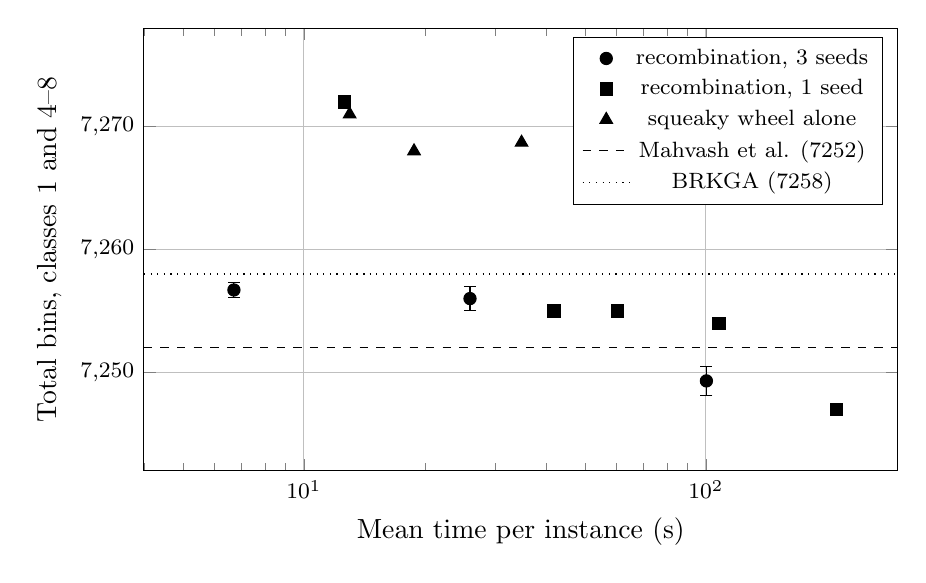
\begin{tikzpicture}
\begin{axis}[width=0.92\textwidth,height=7.2cm,xmode=log,xmin=4,xmax=300,ymin=7242,ymax=7278,
  xlabel={Mean time per instance (s)},ylabel={Total bins, classes 1 and 4--8},grid=major,
  legend style={font=\footnotesize,at={(0.98,0.98)},anchor=north east},tick label style={font=\footnotesize}]
\addplot[only marks,mark=*,mark size=2.2pt,error bars/.cd,y dir=both,y explicit]
  coordinates {(6.7,7256.7) +- (0,0.6) (25.9,7256.0) +- (0,1.0) (100.3,7249.3) +- (0,1.2)};
\addlegendentry{recombination, 3 seeds}
\addplot[only marks,mark=square*,mark size=2.2pt] coordinates {(12.6,7272) (41.9,7255) (60.2,7255) (107.8,7254) (211.3,7247)};
\addlegendentry{recombination, 1 seed}
\addplot[only marks,mark=triangle*,mark size=2.6pt] coordinates {(13,7271) (18.8,7268.0) (34.8,7268.7) (103.7,7267)};
\addlegendentry{squeaky wheel alone}
\addplot[dashed,no marks,domain=4:300] {7252};
\addlegendentry{Mahvash et al. (7252)}
\addplot[dotted,no marks,domain=4:300] {7258};
\addlegendentry{BRKGA (7258)}
\end{axis}
\end{tikzpicture}
\caption{Total bins against mean time per instance on the 240 original instances. Circles: \cfgfast{}, \cfgbal{}
and \cfgqual{} (three seeds, bars: standard deviation; all three from the campaigns of November 2026). Squares, one seed: budget 10 s with recombination
limit 20 s, a run with $T=33$ s and $T_{\mathrm{milp}}=60$ s, and runs of $T=50$ and $T=100$ with the harvest, and $T=200$
(Table~\ref{tab:e-budget}). Triangles: squeaky wheel alone with the time given (13, 18.8, 34.8 and 103.7 s; the second
with two seeds, the third with three, the others with one). The horizontal lines are totals from the literature,
whose times are not comparable.}
\label{fig:e-curve}
\end{figure}

Two observations qualify the table. First, the harvest helps with small budgets and not with large ones: with
$T=100$ and the harvest the result (7254, one seed) is above that of \cfgqual{} without it (7249 in that seed of the earlier campaign; worse in 7
instances and better in 2, $p=0.18$), which agrees with the explanation that a larger pool makes the MILP harder under a fixed time
limit. Second, the runs with one seed are subject to the variation between seeds, whose standard
deviation on the total is 0.6, 1.0 and 1.2 bins for \cfgfast{}, \cfgbal{} and \cfgqual{} (and 3.5 for \cfgfast{} without the harvest, in the repetition); as noted above, the variation
between campaigns can be larger than that.
\paragraph{Time per instance.}
The limits bound the time of the two phases, but the recombination uses time up to its limit in a few runs, so the
mean exceeds the median: \cfgfast{} has a median of 4.2 s, a mean of 6.7 s and a maximum of 34.2 s, and \cfgbal{}
20.5, 25.9 and 80.4 s. The MILP reaches its limit without a proof in 4.6\% to 7.9\% of the runs. Anyone who needs a
bound on the running time should read the maximum, $T+T_{\mathrm{milp}}$ plus one construction. The distribution is in
Table~\ref{tab:e-time} (Appendix~\ref{app:tables}).

\subsection{Comparison with the literature, rotations}
\label{sec:e-rot}

\pend{All the rows of this section come from campaigns whose raw files were lost. Repeat \cfgfast{},
\cfgbal{}, \cfgqual{}, the configuration with $T=33$ and the matched squeaky wheel loop on the 320 instances
with rotations under the protocol of Section~\ref{sec:e-setup}; this is the strongest comparison of the paper.}

With rotations the blocks include the six orientations; nothing else changes. Table~\ref{tab:e-rot} gives the results and the totals of
\citet{Mahvash2018} (Table~1 of their article, sum of the averages of their cells times ten; the total of 6854 for classes 1 and 4--8 is computed by us from their rows, and the
total of 9013 for the eight classes is the one they print) and of BRKGA with six orientations \citep{Goncalves2013}. The BRKGA values for 200 boxes in classes 6, 7 and 8 are below the lower bound with
rotations, which cannot happen for averages of valid solutions of the same instances, so we do not use that total as a reference.

\begin{table}[t]
\centering
\small\setlength{\tabcolsep}{4pt}
\caption{Total bins with rotations (six orientations). Ours: mean and standard deviation over three seeds; time per instance in brackets. All our rows come from earlier campaigns (two to five runs in parallel, raw files not kept), and the rows of different configurations were not run in the same campaign. $^{a}$ Time limit equal to the mean time of the $T=33$ configuration.}
\label{tab:e-rot}
\begin{tabular}{@{}lrrr@{}}
\toprule
Method & Classes 1, 4--8 (240) & Classes 2, 3 (80) & All classes (320)\\
\midrule
Squeaky wheel alone, matched time$^{a}$ & 6845.3 (39 s) & 2165.0 (57 s) & 9010.3\\
\cfgfast{} & $6840.0\pm 1.0$ (7.2 s) & --- & ---\\
\cfgbal{} & $6840.0\pm 3.0$ (26.5 s) & --- & ---\\
$T=33$, $T_{\mathrm{milp}}=60$, without harvest & $6835.3\pm 1.2$ (43 s) & $2159.0\pm 1.0$ (57 s) & 8994.3\\
\cfgqual{} & $6831.0\pm 2.0$ (98.2 s) & $2154.3\pm 0.6$ (117.4 s) & 8985.3\\
\midrule
\citet{Mahvash2018} & 6854 & 2159 & 9013\\
BRKGA, \citet{Goncalves2013} & 6837 (not reliable) & 2172 & 9009\\
\bottomrule
\end{tabular}
\end{table}

\cfgqual{} obtains 8985.3 bins on the eight classes against 9013 of \citet{Mahvash2018}, 27.7 bins (0.31\%) fewer, in 98.2 and 117.4 s per instance against a time per instance
of a few seconds to under 1000 s on their machine (about 310 s on average over the 32 rows of their Table~1). Cell by cell, in classes 1 and 4--8 it is below their total in 12 of the 24 cells, equal in 10 and above in 2; in
classes 2 and 3 it is below in 6 cells and above in 2 (class 2 and class 3 with 200 boxes: 42.13 against 41.9 and 42.17 against 42.1). \cfgbal{} is below in 11, equal in 9 and above in 4
of the 24 cells of the first group. With rotations the larger budget does pay: \cfgqual{} is nine bins below \cfgbal{} in classes 1 and 4--8, better in 10, 12 and 8 instances per seed and worse in 0, 1 and 2
($p=0.0016$, $0.0023$ and $0.058$). The recombination also contributes here: the configuration with $T=33$ is 10.0 bins below the squeaky wheel alone
in classes 1 and 4--8 ($p=0.0027$, $0.0455$ and $0.0075$ by seed), and 6.0 in classes 2 and 3, where the difference per seed is not significant at the 5\% level ($p=0.125$, $0.109$ and $0.065$).
\cfgfast{} also improves on the squeaky wheel alone with rotations (6840.0 against 6845.3) although $\tau=0.005$ s was set for fixed orientation.

\subsection{Contribution of the components}
\label{sec:e-ablation}

\pend{Replace Table~\ref{tab:e-ablation} with the repetition under the protocol
(three seeds, raw files in \texttt{results/bpp/ablation\_2026-11}), which adds a squeaky wheel loop with
$T=26$ s as a control with the same time as the configuration with recombination and harvest. The table is
generated by \texttt{problems/clp/experiments/table\_ablation.py} from the raw files.}

Table~\ref{tab:e-ablation} adds the components one at a time on the 240 original instances with the same search budget
($T=20$ s, $\tau=0.005$ s). The construction with profit $v^2$ (without squeaky wheel) gives 7383.5 bins in 0.1 s per instance; with $\kappa=1$,
that is, maximizing the volume of each bin, it gives 7608.5, and is worse in 151 or 152 of the 240 instances depending on the seed. The squeaky
wheel loop reduces the total by 115.5 bins ($p\approx 10^{-23}$). The learning matters: with $\rho=0$,
where the loop only adds noise, the total is 7307.5, 39.5 bins above the loop with learning. The recombination removes 10 more bins ($p=0.0075$ and $0.0039$
in the two seeds), and the harvest 5.5 more ($p=0.058$ and $0.059$): in this protocol the effect of the harvest is borderline in each seed.
The total reduction from the plain construction to \cfgbal{} is 131 bins, 1.8\%. This ablation is from the earlier campaign, whose raw files were lost; its last row (7252.5) is
3.5 bins below the repetition of \cfgbal{} (7256.0 with the same options), so the effects of the last two components, 10 and 5.5 bins, are reliable only as orders of magnitude;
the effect of the harvest was measured again in the repetition (Table~\ref{tab:e-harvest}).

\begin{table}[t]
\centering
\small\setlength{\tabcolsep}{4pt}
\caption{Ablation on the 240 original instances (fixed orientation, $T=20$ s, $\tau=0.005$ s, two seeds; earlier campaign, raw files not kept).
Each row adds a component to the previous one except the rows marked with $\ast$.}
\label{tab:e-ablation}
\begin{tabular}{@{}lrrrr@{}}
\toprule
Configuration & Bins, seed 1 & Bins, seed 2 & Mean & Time (s)\\
\midrule
Construction, $\kappa=2$ & 7384 & 7383 & 7383.5 & 0.1\\
$\ast$ Construction, $\kappa=1$ & 7613 & 7604 & 7608.5 & 0.1\\
+ squeaky wheel loop & 7269 & 7267 & 7268.0 & 18.8\\
$\ast$ squeaky wheel without learning ($\rho=0$) & 7312 & 7303 & 7307.5 & 19.0\\
+ recombination ($T_{\mathrm{milp}}=60$) & 7259 & 7257 & 7258.0 & 24.4\\
+ harvest ($K=10$, \cfgbal{}) & 7253 & 7252 & 7252.5 & 25.8\\
\bottomrule
\end{tabular}
\end{table}

The effect of the harvest depends on the budget. With the budget of \cfgfast{} (Table~\ref{tab:e-harvest}), adding it to the same configuration
(7266.0 without it) lowers the total to 7256.7, 9.3 bins (0.13\%; $p=0.0002$ on the means of the instances) with 0.9 s more per instance. The squeaky wheel loop alone is not changed
(the totals before the recombination are 7275.0 without the harvest and 7277.3 with it); the whole gain is in the recombination, which removes on average 20.7 bins with the harvest and 9.0
without it. The recombination improves the solution in 8.6\% of the runs with the harvest and in 3.8\% without it. In an earlier campaign with the same
configuration the totals were 7269.7 and 7259.3 (difference $-10.3$; by seed $-14$, $-4$, $-13$). With rotations, \cfgfast{} without harvest obtains $6846.3\pm 3.8$ and with it $6840.0\pm 1.0$ (difference $-6.3$, $p=0.018$;
by seed $-10$, $-1$ and $-8$).

\begin{table}[t]
\centering
\small\setlength{\tabcolsep}{4pt}
\caption{Effect of the harvest at the budget of \cfgfast{} ($T=4$ s, $\tau=0.005$ s, $T_{\mathrm{milp}}=30$ s; 240 original instances; repetition of November 2026).}
\label{tab:e-harvest}
\begin{tabular}{@{}lrrrrr@{}}
\toprule
 & Seed 1 & Seed 2 & Seed 3 & Mean $\pm$ sd & Time (s)\\
\midrule
Without harvest & 7270 & 7264 & 7264 & $7266.0\pm 3.5$ & 5.8\\
With harvest ($K=10$) & 7257 & 7256 & 7257 & $7256.7\pm 0.6$ & 6.7\\
Difference & $-13$ & $-8$ & $-7$ & $-9.3$ & $+0.9$\\
$p$ (Wilcoxon, per seed) & 0.0003 & 0.021 & 0.035 & & \\
\bottomrule
\end{tabular}
\end{table}

Inside the runs of the repetition, comparing the incumbent of the squeaky wheel loop with the final solution,
the recombination removes 8 to 22 bins per seed over the 240 instances, in every seed and configuration ($p<0.005$),
and never worsens a solution (Table~\ref{tab:e-within}, Appendix~\ref{app:tables}). This does not show that its time
is better spent than in the squeaky wheel loop; the matched-time controls of Section~\ref{sec:e-recomb} do.

\paragraph{Parameters of BSG.}
The parameters of BSG were not retuned for bin packing, and the following test shows that the construction does not depend on them. On 120 generated instances (classes 1 and 4--8,
sizes 50 to 200, five instances each) with the construction alone, we varied one parameter at a time: $f_{\min}$ from 0.8 to 1.0, $N_{\max}$ from 100 to 4000, $\alpha$ from 0 to 4, $\beta$
from 0.5 to 4.75, $\gamma$ from 0 to 1 and $p$ from 0 to 0.088. All the totals were within 3 bins of 3649 ($\pm 0.08\%$). We also drew 24 random combinations of all the parameters; the totals
had mean 3649.9, standard deviation 3.0 and range 3645 to 3656, against 3650 for the default values, and the parameters tuned for the ULD problem gave 3653. What changes the result is the choice of the profits (the exponent $\kappa$,
Table~\ref{tab:e-ablation}) and the squeaky wheel loop, not the parameters of the evaluation function.

\subsection{Behaviour of the recombination}
\label{sec:e-recomb}

\paragraph{Effect in several samples.}
Table~\ref{tab:e-milp} compares the squeaky wheel followed by the recombination with the squeaky wheel alone with the same mean time.
The gain is between 10 and 13 bins (0.14\% to 0.43\%) in the samples where the control has about the time of the recombination or, for \cfgfast{} on the first blind set, five times more; on the second blind set the control with four times the time of \cfgfast{} is 6 bins above. Only the classes 2 and 3 and the two blind sets are independent of the design; the
first set of generated instances (240) was used to choose the exponent $\kappa$ and the parameters of BSG (not the budgets of the recombination), and the original
instances decided the configuration. The recombination mixes patterns that the loop itself created, which no iteration of the loop could mix. It does not make a solution worse in the campaigns that we measured, because
it starts from the best solution, but the improvement is rare: in classes 2 and 3 and in the 240 generated instances it saved a bin in 17 of 80 and 17 of 240 instances in at least one seed,
and in 9 to 13 instances per seed.

\begin{table}[t]
\centering
\small\setlength{\tabcolsep}{4pt}
\caption{Total bins of the squeaky wheel alone (``Alone'') and of the squeaky wheel followed by the recombination (``With recomb.''), the first with a time limit close to the mean time of the second except where noted. Each row is one campaign in which the two columns were run
under the same conditions; the campaigns differ from one another (Table~\ref{tab:e-conditions} and the text of Section~\ref{sec:e-setup}), so the rows are compared inside the row and not across rows. The configuration with recombination is
$T=33$ s, $T_{\mathrm{milp}}=60$ s, without harvest, except where noted. $^\dagger$ The result on the original instances was obtained with a prototype in which the
same MILP was solved from Python with HiGHS; the C++ implementation gave 7255 in one seed and the same total in 237 of the 240 instances. In this row the control ran 34.8 s
against 42.8 s for the configuration with recombination; in the other rows with $T=33$ and in the row of \cfgbal{} the times differ by less than 3 s, and in the rows of \cfgfast{} the control ran 35.3 s against 7.3 s (blind set) and 25.3 s against 6.9 s (blind set 2).}
\label{tab:e-milp}
\begin{tabular}{@{}lrrrrr@{}}
\toprule
Sample & Seeds & Alone & With recomb. & Diff. & $p$\\
\midrule
Classes 2 and 3 (80), held out & 5 & 2527.8 & 2517.0 & $-10.8$ & 0.0002\\
Blind set (128), $T=33$ & 3 & 3941.3 & 3930.7 & $-10.7$ & 0.0004\\
Blind set (128), \cfgfast{} & 3 & 3941.3 & 3931.3 & $-10.0$ & 0.0007\\
Blind set 2 (128), \cfgbal{} & 1 & 3893 & 3882 & $-11$ & 0.0010\\
Blind set 2 (128), \cfgfast{} & 1 & 3893 & 3887 & $-6$ & 0.15\\
First generated set (240) & 3 & 7253.0 & 7242.7 & $-10.3$ & 0.0003\\
Original instances (240)$^\dagger$ & 3 & 7268.7 & 7256.0 & $-12.7$ & 0.0001\\
\bottomrule
\end{tabular}
\end{table}

By class (Figure~\ref{fig:e-class}, Appendix~\ref{app:tables}), the gain is concentrated in class 1: in the first set of generated instances the recombination saves 7.0 bins in class 1, 2.0 in class 8, 1.0 in classes 5 and 6, 0.3 in class 7 and none in class 4
(these differences are with respect to the squeaky wheel of 33 s that the recombination starts from). In classes 2 and 3 it saves 6.6 and 4.0.
For the ten instances of class 4 with 50 boxes we enumerated the feasible loads of at most four boxes (checking that
five boxes do not change the result in four instances) and solved the exact cover: it gives 294 bins, the same total as our solver. This suggests that there is nothing to gain in that cell, although we did not prove that no bin can hold more boxes
than the ones enumerated.

\paragraph{Second blind set.}
We measured the recombination on a second blind set of 128 instances (Section~\ref{sec:e-setup}) that we generated for this purpose with registered seeds. Each configuration of
Table~\ref{tab:e-recomb} (Appendix~\ref{app:tables}) was run once on every instance; all the solutions are valid and the raw files are kept. The lower bound of the 128 instances adds up to 3656.

With the budget of \cfgbal{} the recombination lowers the total from 3893 (squeaky wheel alone with the same time) to 3882: $-11$ bins, better in 11 instances and worse in none ($p=0.0010$), a gain
of the size seen in the other samples (Table~\ref{tab:e-milp}). \cfgfast{}, with a quarter of the time, obtains 3887 ($-6$ with respect to the squeaky wheel alone, $p=0.15$), and removing the harvest from it gives 3893 ($+6$, $p=0.11$);
with one seed neither of these two differences is significant. The harvest multiplies the pool by 7.5 (467 to 3493 columns on average).

\paragraph{Cost of the recombination.}
The recombination is cheap in most instances (Figure~\ref{fig:e-outcome}). With \cfgbal{}, the LP of the pool proves in 113 of the 128 runs (88\%) that the pool has no solution with fewer bins than the incumbent, and in 101 of them (79\% of the runs) the first
LP is enough and no MILP is solved. The MILP proves it in nine more runs, so 122 runs (95\%) end with a proof for the pool, and the MILP improves the solution in 12 (9.4\%). In six runs (4.7\%) the MILP reaches its limit of 60 s without a proof
and without an improvement, and they use 54\% of the total time of the MILPs (360 of 661 s). \cfgfast{} behaves in the same way (95\% of the runs proven, 10.9\% improved, 7 unproven runs with 56\% of the MILP time). On 192 instances used during the development,
with the configuration of 33 s, the corresponding figures were 94\%, 12.5\% and 6\%.

\begin{figure}[t]
\centering
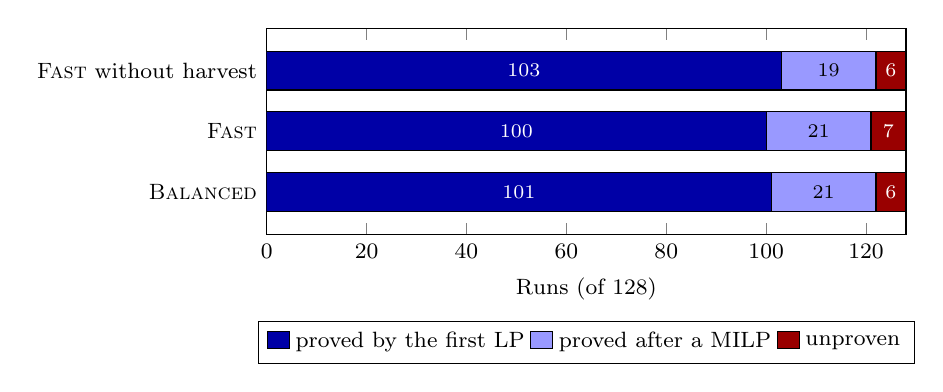
\begin{tikzpicture}
\begin{axis}[xbar stacked,width=0.8\textwidth,height=4.2cm,xmin=0,xmax=128,ytick={0,1,2},y dir=reverse,
  yticklabels={{\cfgfast{} without harvest},{\cfgfast{}},{\cfgbal{}}},xlabel={Runs (of 128)},bar width=14pt,ymin=-0.7,ymax=2.7,
  legend style={font=\footnotesize,at={(0.5,-0.42)},anchor=north,legend columns=3},tick label style={font=\footnotesize},label style={font=\footnotesize},
  nodes near coords,every node near coord/.append style={font=\scriptsize,text=white}]
\addplot[fill=blue!65!black] coordinates {(103,0) (100,1) (101,2)};
\addlegendentry{proved by the first LP}
\addplot[fill=blue!40!white,nodes near coords style={text=black}] coordinates {(19,0) (21,1) (21,2)};
\addlegendentry{proved after a MILP}
\addplot[fill=red!60!black] coordinates {(6,0) (7,1) (6,2)};
\addlegendentry{unproven}
\end{axis}
\end{tikzpicture}
\caption{How the runs of the second blind set end: the first LP of the pool proves that the incumbent is the best of the pool, a MILP is needed and then the LP or the MILP proves it, or the MILP reaches
its time limit without a proof.}
\label{fig:e-outcome}
\end{figure}

The LP of the pool also bounds what a recombination can obtain from its columns. With \cfgbal{}, the sum of the rounded LP values is 3867 and the solutions add up to 3882 bins: in 113 instances the
solution equals the rounded LP value and in 15 it exceeds it by one, so at most 15 bins (0.4\%) could be gained with these pools. The figures are 3873 against 3887 for \cfgfast{} (114 and 14 instances) and 3877 against 3893 for \cfgfast{} without harvest. A better pool, not a better recombination, is
then the way to improve; this agrees with the 0.9\% bound that we obtain on large instances (Section~\ref{sec:e-scale}).

\paragraph{LP bound and reduced-cost fixing.}
The saving of time comes mainly from the LP bound and little from the fixing. A MILP stage was needed in 27 of the 128 runs of \cfgbal{}, and in them the fixing kept on average 86\% of the columns (median 96\%): when the LP
leaves a gap with respect to the incumbent, few columns can be discarded. The plain MILP (warm start, without LP proof and without fixing) with the same budget takes 17.1 s per instance on average against 5.2 s of the version with LP proof and fixing
(total 2190 s against 661 s, $-70\%$), and obtains 3884 bins against 3882. The difference in time is concentrated in the 60 runs in which the plain MILP needs more than 5 s (2107 s against 634 s). The two runs of an instance do not
share exactly the same pool, because the clock changes the search of BSG, so this compares the two procedures and not the two models over one pool. We do not report a separate measurement of the fixing alone.

\subsection{Generalisation: held-out classes and blind sets}
\label{sec:e-heldout}

Classes 2 and 3 were never used to choose a configuration. We ran on them the configuration that we had then
(squeaky wheel of 33 s followed by the recombination with a limit of 60 s, without harvest) and of \cfgfast{}. The
standard deviation of this configuration (1.4) is the sample one, computed from the five totals 2519, 2517, 2515, 2517 and 2517. The
recombination saves 10.8 bins (0.43\%) with respect to the squeaky wheel alone with the same time (Wilcoxon $p=0.0002$ over five seeds); in each
seed it improves 10 to 14 instances and worsens none. This configuration obtains 2517.0, below the totals published for BRKGA (2519), GVND (2527) and TS3 \citep{Lodi2002}
(2543), and above the total of \citet{Mahvash2018} (2514). \cfgfast{} obtains 2521.0, four bins above the longer configuration, with 5.4 times less
time. We did not run \cfgbal{} and \cfgqual{} on these classes without rotation.

The blind set confirms the two effects. \cfgfast{} (3931.3) is 0.7 bins above the configuration with $T=33$ (3930.7, $p=0.16$) with five
times less time, and both are about ten bins below the squeaky wheel alone with the time of the second (3941.3):
$-10.0$ ($p=0.0007$) and $-10.7$ ($p=0.0004$). Removing the harvest from \cfgfast{} raises the total by 4.7 bins ($p=0.011$ on the means of
the instances; per seed $+4$, $+5$, $+5$ with $p=0.046$, $0.096$ and $0.025$). That is a smaller effect than on the original instances (below).

\subsection{Vertical support: industrial instances}
\label{sec:e-ind}

\pend{The large instances use the construction alone, as when the recombination was believed to be incompatible
with support. With the partitioning model the whole pipeline applies: run, at the same time per instance
($\approx 18$ s and $\approx 60$ s), the construction alone with $\tau=2$ s against the squeaky wheel loop with
$\tau\in\{0.2,0.5\}$ s, with and without the partitioning recombination. The instances, their converter and the
support validator must be added to the repository.}

\paragraph{Configuration.}
These instances have 50 to 2000 boxes and bins that hold more than a hundred boxes when $n\ge 500$. We require, on every box above the floor, that at least 70\% of its
base rests directly on boxes (Section~\ref{sec:m-ext}). In the runs reported here, for $n\ge 500$ we use the construction alone, with $\kappa=1$ and $\tau=2$ s per bin.
These values were chosen by looking at a few instances of this benchmark (the first instance of each class with $n=1000$, the second instance of classes 1 and 2 with $n=500$, the first instance of class 1 with $n=500$ and 2000 and eight
instances of classes 3 and 4 with $n=1500$ and 2000); the choice is not independent of the benchmark.

\paragraph{Comparison with LCGA.}
Table~\ref{tab:e-ind} gives the mean number of bins per cell for $n\ge 500$, with one run per instance, against the values of \citet{Elhedhli2019} (Table~9 of their article). The total over the 16 cells is 144.6 bins against 153.6 (5.9\% fewer):
we are below in 11 cells, equal in 5 and above in none (exact sign test, $p=0.0010$; the cells share a configuration and a choice of parameters, so the test is descriptive). Three runs of the whole set (the construction is deterministic except for the clock) gave 723, 721 and 723 bins in the 80 instances,
that is, 722.3 on average (144.5 as a sum of cell means), and in each run 80 of 80 solutions satisfy the 70\% support in every box (independent check of geometry and support). The time per instance is 18.3 s on average with two runs in parallel, against 608 s for LCGA;
that is 33 times less in raw time and about 15 times after a factor of 2.27 between the single-thread ratings of the two processors \citep{PassMark} (3740 for the i5-14400 and 1650 for the i7-5500U; the factor is approximate). In the instances 3 to 5 of each cell, which were not looked at while choosing $\kappa$ and $\tau$, the excess over the lower bound
is 0.92 bins per instance for our method and 1.46 for LCGA (compared by cell averages because the numbering differs).

\begin{table}[t]
\centering
\small\setlength{\tabcolsep}{4pt}
\caption{Industrial instances, $n\ge 500$: mean number of bins per cell (five instances), ours with one run per instance and two runs in parallel at below-normal priority (construction alone, $\kappa=1$,
$\tau=2$ s, support 70\%) and LCGA \citep{Elhedhli2019}.}
\label{tab:e-ind}
\begin{tabular}{@{}lrrrrrrrr@{}}
\toprule
 & \multicolumn{4}{c}{Ours} & \multicolumn{4}{c}{LCGA}\\
\cmidrule(lr){2-5}\cmidrule(lr){6-9}
Class & 500 & 1000 & 1500 & 2000 & 500 & 1000 & 1500 & 2000\\
\midrule
1 & 4.0 & 8.2 & 12.0 & 16.0 & 5 & 8.8 & 12.4 & 16\\
2 & 4.0 & 8.0 & 12.0 & 16.0 & 5 & 9 & 12 & 16\\
3 & 4.0 & 7.0 & 10.0 & 13.0 & 4 & 7 & 10.6 & 14\\
4 & 3.4 & 6.0 & 9.0 & 12.0 & 4 & 7 & 10 & 12.8\\
\midrule
Sum & \multicolumn{4}{c}{144.6} & \multicolumn{4}{c}{153.6}\\
\bottomrule
\end{tabular}
\end{table}

Three caveats limit this comparison. The instances are from the same distribution but we could not verify that they are those of the article. The support: LCGA does not impose it on every box in its main results; its columns of supported items
in the appendix tables give 78.2\% of the boxes with at least 70\% support (83.2\% for $n\ge 500$) and a mean support of 92.3\% for $n\ge 500$ (our reading of their tables), while we impose 70\% on every box and obtain a mean support of 90.5\% to 92.6\%. This
makes our requirement the stricter one. Last, \citet{Elhedhli2019} allow a tolerance of 5 mm in the heights when forming layers, and we require exact contact.

\paragraph{Time per bin and $\kappa$.}
On the 48 instances obtained by resampling and the 24 from the catalogue (Table~\ref{tab:e-indnew}, Appendix~\ref{app:tables}), the default configuration for the Martello et al.\ instances ($\kappa=2$, $\tau=0.02$ s) gives 497 and 264 bins; the
configuration of this section ($\kappa=1$, $\tau=2$ s) gives 438 and 233, 11.9\% and 11.7\% fewer, but with 18 s per instance instead of less than one second. The fair control is the one that keeps $\tau=2$ s and
$\kappa=2$: it gives the same 438 bins in the resampled instances (4 instances better, 4 worse, 40 equal) and 241 in the catalogue instances, eight bins more (3.3\%) than $\kappa=1$ (better in 8, worse in none). Most of the gain thus
comes from the time per bin, and $\kappa=1$ helps only in the catalogue instances.

\paragraph{Cost of the support requirement.}
Table~\ref{tab:e-support} shows the construction with $\kappa=1$ and $\tau=2$ s on the 80 instances with $n\ge 500$ for several support criteria. Requiring 70\% on every box costs 15 bins out of 708 (2.1\%) with respect to requiring nothing; without a requirement, only 77.3\% of
the boxes have 70\% of support, so the explicit condition is necessary. Stricter criteria are costly: 85\% costs 9.7\% more than 70\%, and full support 80\% more. We
also tried 95\% and 100\% of the base on eight instances (classes 1--4, first instance, $n=500$ and 1000): 43\% and 89\% more bins than 70\% (the total of the eight was 63 and 83 against 44), so the cost does not appear only with full support. We did not determine whether the block structure of the
generator or the criterion itself is the cause.

\begin{table}[t]
\centering
\small\setlength{\tabcolsep}{4pt}
\caption{Criteria of support (industrial instances, $n\ge 500$, 80 instances, construction alone, $\kappa=1$, $\tau=2$ s, one run per instance, two runs in parallel). Support: percentage of the base area resting on boxes.}
\label{tab:e-support}
\begin{tabular}{@{}lrrrrr@{}}
\toprule
Criterion & Bins & Time (s) & Mean support & Boxes with $\ge 70\%$ & Boxes fully supported\\
\midrule
None & 708 & 17.3 & 80.4\% & 77.3\% & 28.3\%\\
50\% of the base & 720 & 17.9 & 88.7\% & 86.9\% & 32.6\%\\
70\% of the base (used) & 723 & 18.3 & 91.4\% & 100\% & 33.0\%\\
85\% of the base & 793 & 19.6 & 95.2\% & 100\% & 37.2\%\\
Full support & 1303 & 32.1 & 100\% & 100\% & 100\%\\
\bottomrule
\end{tabular}
\end{table}

\paragraph{Small industrial instances.}
For $n<500$ the construction alone leaves one or two bins per cell and is not better than LCGA (23.4 against 23.0 bins over the 16 cells). With a configuration that also includes the improvement phase of Appendix~\ref{app:improve}
($T=30$ s, 30\% of it for the squeaky wheel loop and the rest for the improvement phase, with the reload from scratch, $\kappa=1$,
$\tau=0.02$ s in the construction and 0.04 s in the improvement phase) the total is 22.0 against 23.0 (below in two cells and equal in 14), with 5 s per instance on average because the search stops when the lower bound is reached.

\subsection{Limits: large instances}
\label{sec:e-scale}

The recombination does not scale to instances with several hundred boxes with the budgets used here. On 36 generated instances with $n=500$ and $n=1000$ (six classes, three instances per class and size), the squeaky wheel followed by the recombination (50 s and 60 s) obtains 6183 bins in 101.5 s,
against 6179 of the squeaky wheel alone with 102 s (the second is better in 5 instances and the first in 1, $p=0.22$). The recombination improves one instance of 36, uses the whole limit of 60 s in almost all of them (50.0 s on average) and works with about 2095 columns.
The lower bounds are 1955 for $n=500$ and 3958 for $n=1000$, against 2056 and 4127 bins of the first configuration. In another set of 24 generated instances (six classes, two sizes with $n=500$ and 1000, two instances each), the pools of \cfgbal{} give
4072 bins, and the sum of the rounded LP values of those pools is 4036: even a perfect recombination of those pools could save at most 36 bins (0.9\%). The margin
is then in the generation of better columns and not in the recombination.

\subsection{Discussion and limits of the evidence}
\label{sec:e-discussion}

\paragraph{What the results support.}
The recombination of the bins produced by the search is the component that is best supported. In the seven comparisons of Table~\ref{tab:e-milp} the squeaky wheel loop alone has a total that is between 6 and 13 bins above that of the
configuration with recombination, including the comparisons in which the control runs four to five times longer than \cfgfast{}, and inside the runs of the repetition the recombination saves bins in every seed and configuration without ever worsening a solution.
Classes 2 and 3 and the two blind sets were not used to take any decision. Without rotations the total of \cfgfast{} and \cfgbal{} is at the level of the best published ones and that of \cfgqual{} is 2.7 bins below the lowest (7249.3 against 7252), and with rotations the long configuration is below the total of \citet{Mahvash2018}.
In the industrial instances the construction alone, with the 70\% support imposed on every box, uses fewer bins than the totals that \citet{Elhedhli2019} report.

\paragraph{Comparison with the literature.}
The totals of the other methods are taken from their articles. They come from other machines and from an unknown number of runs, and \citet{Mahvash2018} do not report times for the experiments without rotation. We normalised the times only
in the industrial comparison, and with a processor rating that is approximate (Section~\ref{sec:e-ind}), so the statements about time with respect to other methods are indicative. We could not apply statistical tests against the literature because the results per instance
are not published. The total of \citet{Mahvash2018} remains below the shorter configurations without rotation. \cfgqual{} is 2.7 bins below it, with a standard deviation of 1.2 bins over seeds and a different machine, and for that reason we do not claim that the method improves the state of the art in that setting.

\paragraph{Variation between campaigns.}
Repeating \cfgfast{} and \cfgbal{} on the original instances with the same code and options gave totals that differ from those of the earlier campaign by 2.6 and 3.0 bins (Section~\ref{sec:e-mpv}), more than the standard deviation between seeds inside a campaign (0.6 to 2.1 bins); \cfgqual{}, in contrast, moved by 0.7 bins (7250.0 against 7249.3).
Because the time limits are wall-clock limits, the load of the machine changes the amount of search that a run receives, and we do not control it. For this reason, differences of a few bins between configurations measured in different campaigns should not be interpreted, and we
mark the figures that come from campaigns whose raw files were lost.

\paragraph{Tuning on the benchmark.}
The exponent $\kappa$ and the budgets were chosen with the original instances and with generated instances of the same distribution. The absolute totals on the original instances are therefore not independent of the design. The effects that matter for the conclusions
were also measured on classes 2 and 3 and on two blind sets, and they have the same sign and a similar size there. In the industrial instances $\kappa$ and the time per bin were chosen with a few instances of the same benchmark, and the 48 additional instances
were obtained by resampling its boxes, so they are not independent either (Section~\ref{sec:e-ind}).

\paragraph{Limits of the method.}
The recombination does not scale to several hundred boxes with the budgets used here: with $n=500$ and $1000$ it improved one instance of 36, and the LP of the pools shows that at most 0.9\% could be gained from them (Section~\ref{sec:e-scale}). The covering model is not compatible with the support requirement,
because removing the surplus boxes can leave a box without support; the partitioning model is, but its effect on the industrial instances is not measured yet, and the results reported for $n\ge 500$ come from the construction alone. The support criterion is expensive when it is made stricter: 85\% of the base costs 9.7\% more bins than 70\%, and full support 80\% more (Table~\ref{tab:e-support}).
The method needs a MILP solver for the recombination; without it only the construction and the squeaky wheel loop are available.

\paragraph{Industrial instances.}
The industrial totals are the mean of five instances per cell with one run per instance. Three complete runs of the 80 instances with $n\ge 500$ gave 723, 721 and 723 bins, so the variation caused by the clock is small: four instances of the 80 changed by one bin between runs,
and the advantage of 5.9\% over LCGA is much larger than that. The instances have the distribution and the structure of those of \citet{Elhedhli2019}, and the lower bound of their cells coincides with ours in 30 of 32, but we could not verify that they are the same
files, and \citet{Elhedhli2019} tolerate 5 mm in the heights when they form layers while we require exact contact.

% Seccion "Conclusions" del paper de bin packing 3D (BSG_BPP).
\section{Conclusions}
\label{sec:conclusions}

We presented a method for the three-dimensional bin packing problem that generates bin patterns with a
single-bin loader inside a squeaky wheel loop over the profits of the box types, enlarges the pool with
the loads that the loader explores and discards, and recombines the pool with a set covering model, or
with a set partitioning model when the bins must respect vertical support. The LP relaxation of the
pool tells when the recombination has nothing more to offer, and in most runs no integer program is
solved.

On the benchmark of \citet{Martello2000} the method is at the level of the best published totals
without rotations and below them with rotations. The squeaky wheel loop gives most of the improvement
over a single construction; the recombination adds a small but consistent saving, also on instances
that were not used to design the method, and the harvest makes it effective with short budgets. On
industrial instances with 70\% support on every box the method uses fewer bins than the column
generation over layers of \citet{Elhedhli2019}.
\pend{Rewrite after the pending experiments: the role of the squeaky wheel loop and of the
partitioning model under vertical support is not measured yet.}

\paragraph{Limits.}
The recombination can only choose among the patterns in the pool. With several hundred boxes the pools
of our budgets leave little room (at most 0.9\% of the bins according to their LP), so the quality
depends on the generation of patterns and not on the recombination. The covering model needs that
removing a box keeps a bin feasible; the partitioning model removes that requirement at the price of a
harder model. The comparisons with the literature are made on totals, from other machines and an
unknown number of runs.

\paragraph{Future work.}
The generator receives no information from the recombination. Using the dual prices of the pool as
profits for BSG, as column generation does, did not pay with our budgets, but it may with longer ones.
Other loading constraints that a single-bin loader can enforce (weight limits, load balance, fragility)
fit the same scheme with the partitioning model.

\appendix
% Apendice del paper de bin packing 3D: resultados por clase y tamano (8 clases, orientacion fija).
% Las filas las genera tools/analysis/table_cells.py desde los resultados de las campanas y las cifras de la literatura.
\providecommand{\todo}[1]{\textcolor{red}{[TODO: #1]}}
\section{Results by class and size}
\label{app:cells}

Table~\ref{tab:e-cells} gives, for each class and size, the sum of the ten instances, with fixed orientation. The columns of our
configurations are the mean of three seeds, rounded to one decimal; the totals are computed with unrounded values. The other columns are published values:
\citet{Mahvash2018} (Table~2 of their article, column generation with a MILP; averages times ten), and, from Table~8 of \citet{Goncalves2013} (averages times ten),
BRKGA, TS3 \citep{Lodi2002}, GVND \citep{Parreno2010}, TS2P \citep{Crainic2009} and GLS \citep{Faroe2003}; the last two were not reported for classes 2 and 3.
The best published value of each cell is in bold. LB is the sum of the lower bounds given in the header of each instance file (6852 for classes 1 and 4--8;
the bound computed by our program, which is the maximum of the continuous bound and the bounds $L_1$ and $L_2$ of \citet{Martello2000}, adds up to 6837 on the same instances).
Classes 2 and 3 were not used to choose any parameter.

\begin{table}[htbp]
\centering
\footnotesize\setlength{\tabcolsep}{3pt}
\caption{Total bins per class and size, 320 original instances, fixed orientation.}
\label{tab:e-cells}
\begin{tabular}{@{}rrrrrrrrrrrr@{}}
\toprule
Class & $n$ & LB & Mahvash & BRKGA & TS3 & GVND & TS2P & GLS & \cfgfast{} & \cfgbal{} & \cfgqual{}\\
\midrule
1 & 50 & 125 & \textbf{134} & \textbf{134} & \textbf{134} & \textbf{134} & \textbf{134} & \textbf{134} & 134 & 134 & 134 \\
1 & 100 & 251 & \textbf{266} & \textbf{266} & \textbf{266} & \textbf{266} & 267 & 267 & 265.7 & 265.3 & 266 \\
1 & 150 & 347 & \textbf{363} & 364 & 367 & 364 & 370 & 370 & 363.7 & 363 & 363 \\
1 & 200 & 484 & \textbf{507} & 508 & 512 & 509 & 511 & 512 & 507 & 507 & 507 \\
2 & 50 & 127 & \textbf{138} & \textbf{138} & \textbf{138} & \textbf{138} & -- & -- & 138 & 138 & 138 \\
2 & 100 & 241 & \textbf{255} & 256 & 257 & 257 & -- & -- & 255.3 & 255 & 255 \\
2 & 150 & 351 & \textbf{364} & 366 & 372 & 369 & -- & -- & 365.3 & 364 & 364 \\
2 & 200 & 475 & \textbf{493} & 494 & 501 & 494 & -- & -- & 494 & 493 & 493 \\
3 & 50 & 123 & \textbf{133} & \textbf{133} & \textbf{133} & \textbf{133} & -- & -- & 133 & 133 & 133 \\
3 & 100 & 247 & \textbf{259} & \textbf{259} & 260 & 260 & -- & -- & 259 & 259 & 259 \\
3 & 150 & 360 & \textbf{374} & 375 & 377 & 376 & -- & -- & 375.3 & 375 & 375 \\
3 & 200 & 478 & \textbf{498} & \textbf{498} & 505 & 500 & -- & -- & 499.7 & 497.3 & 497 \\
4 & 50 & 289 & \textbf{294} & \textbf{294} & \textbf{294} & \textbf{294} & \textbf{294} & \textbf{294} & 294 & 294 & 294 \\
4 & 100 & 576 & 590 & 590 & 590 & 590 & \textbf{589} & 590 & 590 & 590 & 590 \\
4 & 150 & 852 & \textbf{868} & \textbf{868} & \textbf{868} & \textbf{868} & \textbf{868} & \textbf{868} & 868 & 868 & 868 \\
4 & 200 & 1163 & \textbf{1188} & \textbf{1188} & \textbf{1188} & \textbf{1188} & \textbf{1188} & 1190 & 1188 & 1188 & 1188 \\
5 & 50 & 74 & \textbf{83} & \textbf{83} & 84 & \textbf{83} & \textbf{83} & \textbf{83} & 83 & 83 & 83 \\
5 & 100 & 129 & \textbf{150} & \textbf{150} & \textbf{150} & \textbf{150} & 152 & 151 & 150 & 149.7 & 149.3 \\
5 & 150 & 174 & \textbf{199} & 200 & 204 & 201 & 201 & 202 & 199 & 199.3 & 199 \\
5 & 200 & 244 & \textbf{270} & 271 & 276 & 271 & 274 & 272 & 270 & 270 & 270 \\
6 & 50 & 91 & 98 & \textbf{97} & 99 & 98 & 98 & 98 & 98 & 98 & 98 \\
6 & 100 & 175 & \textbf{189} & \textbf{189} & 191 & 190 & 191 & 191 & 188.3 & 188.7 & 188 \\
6 & 150 & 269 & 292 & \textbf{290} & 294 & 292 & 292 & 294 & 291.3 & 291.3 & 290 \\
6 & 200 & 350 & \textbf{372} & 373 & 377 & 374 & 377 & 377 & 373 & 373 & 372.7 \\
7 & 50 & 64 & \textbf{74} & \textbf{74} & 75 & \textbf{74} & \textbf{74} & \textbf{74} & 74 & 74 & 74 \\
7 & 100 & 109 & 123 & \textbf{122} & 125 & 125 & 123 & 123 & 123 & 123.3 & 122.7 \\
7 & 150 & 137 & 154 & \textbf{153} & 161 & 160 & 158 & 158 & 153 & 153 & 152.3 \\
7 & 200 & 210 & \textbf{232} & 234 & 239 & 235 & 235 & 235 & 234 & 234 & 233.7 \\
8 & 50 & 83 & \textbf{92} & \textbf{92} & 93 & \textbf{92} & \textbf{92} & \textbf{92} & 92 & 92 & 92 \\
8 & 100 & 176 & 189 & 189 & 189 & 189 & \textbf{188} & 189 & 189 & 189 & 189 \\
8 & 150 & 213 & \textbf{235} & 236 & 241 & 241 & 239 & 239 & 234 & 234.3 & 234 \\
8 & 200 & 267 & \textbf{290} & 293 & 303 & 298 & 300 & 299 & 294.7 & 294 & 291.7 \\
\midrule
Total, classes 1 and 4--8 &  & 6852 & 7252 & 7258 & 7320 & 7286 & 7298 & 7302 & 7256.7 & 7256 & 7249.3 \\
Total, classes 2 and 3 &  & 2402 & 2514 & 2519 & 2543 & 2527 & -- & -- & 2519.7 & 2514.3 & 2514 \\
\bottomrule
\end{tabular}
\end{table}

\section{Variants that did not improve the method}
\label{app:negative}
\label{sec:e-negative}

We tried other changes during the development. None of them is part of the method, and we list them because they delimit what can be expected from this approach. The tests were run
with earlier versions of the code, with fewer seeds and on the sets used for development (the 72 original instances of classes 1 and 4--8 with sizes 50 to 200 and the first three instances of each cell,
unless the table says otherwise), and the raw files of some of them were not preserved. The numbers are those obtained then.

\begin{table}[t]
\centering
\small\setlength{\tabcolsep}{4pt}
\caption{Variants tested and discarded. ``Base'' is the method without the variant under the same budget.}
\label{tab:e-negative}
\begin{tabular}{@{}p{3.7cm}p{4.0cm}p{7.2cm}@{}}
\toprule
Variant & Test & Result\\
\midrule
Swaps and transfers of one or two boxes between two bins, accepted by the sum of squares of the loads & 72 original instances, $T=10$ s, five seeds & 2181.4 against 2178.0 for the base ($+3.4$, $p=0.038$); it removes zero to two bins in the 72 instances\\
Random subset of boxes for each bin (a multiple $r$ of the volume of the bin) & same, two seeds & $r=2$: 2281.0 ($+4.7\%$); $r=1.5$: 2330.5 ($+7\%$)\\
Random exponent $\kappa$ at each iteration of the loop & same, three to five seeds & spread 0.5: 2178.8 ($p=0.53$); spread 1: 2181.0 ($+3.0$, $p=0.042$)\\
Keep the weights of the incumbent (undo the update when the solution is worse) & same, two seeds & 2184.5 against 2178.0 ($p=0.023$)\\
Geometric prior on the profit of the boxes & same, three seeds, $T=10$ s & 2177.7 and 2178.7 against 2178.0 ($p=0.75$ and $0.35$)\\
Improvement phase (Appendix~\ref{app:improve}) instead of squeaky wheel & 72 generated instances, about 20 s & construction 2172; with the improvement phase 2168; squeaky wheel loop 2139; half of the time for each 2142\\
Column generation with dual prices as profits for BSG, then the MILP & 240 original instances, three seeds & 7263.7 with squeaky wheel 10 s, generation 20 s and MILP 60 s, against 7256.0 with squeaky wheel 33 s and MILP 60 s ($p=0.0011$)\\
Squeaky wheel loop guided by the dual prices & 36 generated instances (classes 1, 5, 8), $T=20$ s & 987 bins against 986 ($p=0.79$)\\
Recombination with a subproblem (large neighbourhood search) & 24 generated instances, 500 and 1000 boxes & 4071 and 4070 against 4072, with 68\% and 87\% more time ($p=0.56$ and $0.32$)\\
Window of the 1000 columns of lowest reduced cost in the MILP & same & 4072 against 4070 with the complete model, 36\% less time\\
Filter of dominated columns & 240 original instances, two seeds & 7254 and 7258 against 7254 and 7257; it removes 16\% of the columns and the MILP time goes from 7.98 to 7.76 s\\
Partition model instead of covering (compatible with support) & 80 small industrial instances & 112 bins with both; they differ in four instances, two for each\\
Repacking of the least loaded bins as a subproblem & bins of the final solutions of the 240 original instances & five bins: 2 of 224 instances improved; eight bins: 0 of 208\\
Union of the pools of the three seeds & 240 original instances, MILP limit 30 s & 7254 bins, against 7253 for the best of the three seeds on each instance\\
\bottomrule
\end{tabular}
\end{table}

Two results are worth stressing. The column generation with dual prices, the usual way to generate patterns, is worse than spending the same time in the squeaky wheel loop and recombining its bins, at least with 20 s for the
generation, which does not tell us how it would behave with a budget of the order of 1000 s as the one of \citet{Mahvash2018}. And the improvement phase that removes a bin by ruin and recreate, effective when the bins have a large slack as in the industrial instances,
loses against giving the time to the squeaky wheel loop in the benchmark of \citet{Martello2000}, where the bins have a slack of about 5\%.
The option that stops the search when the LP of the pool proves the incumbent optimal for the pool is not a negative result but a trade of quality for time: on 192 generated instances it reduces the mean time by 14\% (31.3 s against 36.2 s) and
increases the total by four bins in 5870 (0.07\%, $p=0.22$), so we do not include it in the three configurations.

\section{Improvement phase for instances with few bins}
\label{app:improve}

\pend{Decide whether this phase stays in the method. It is used only for the small industrial instances; if the squeaky wheel loop with the partitioning model matches it there, remove it.}

When a solution has only a few bins, as in the small industrial instances, the search can be
followed by a phase that tries to remove one bin. It receives the part of the time limit $T$ that
the squeaky wheel loop does not use (30\% of $T$ goes to the loop and 70\% to this phase in the
experiments on small industrial instances); in the three configurations of Table~\ref{tab:configs}
the loop uses all of $T$ and the phase does not run. The bins are taken as target one at a time,
from the least loaded, and the boxes of the target are the pending boxes to be inserted into the
other bins. For each fraction $\phi\in\{0.3,0.6,0.9\}$ and for each of the other bins, again from
the least loaded, boxes with no box above them are removed, highest first, until a fraction $\phi$
of the loaded volume of the bin is out. BSG then reloads the bin with the remaining boxes fixed in
their positions and the pending boxes available, and the new load replaces the old one if it has
more profit (ties are broken by volume). As an option, every bin is first reloaded from scratch with
its boxes and the pending ones, with the same acceptance rule. If every pending box is inserted, the
target disappears. Otherwise, if BSG can load all the pending boxes in one bin and the sum of the
squares of the loaded volumes increases, the change is accepted, because it prepares the removal of
a bin in the next attempts. When a complete pass over the targets changes nothing, the boxes
removed and the fraction $\phi$ (uniform in $[0.2,0.9]$) are drawn at random instead. The phase
stops when the number of bins reaches $\mathrm{LB}$ or the time is over. The calls to BSG in this
phase last $\mu\tau$, with $\mu=2$ in the experiments on small industrial instances. On the other
instances the phase did not improve the results (Section~\ref{sec:e-negative}).

\bibliographystyle{plainnat}
\bibliography{references}
\end{document}
